%!TEX program = lualatex
%!TEX encoding = UTF-8 Unicode  
%!TEX root = chapter11.tex  
\documentclass[main.tex]{subfiles}
\begin{document} 
%----------------------------------------------------------------------------------------
%	CHAPTER  
%----------------------------------------------------------------------------------------
\cleardoublepage
\loadgeometry{marginlayout}  
\pagestyle{scrheadings} % Print headers again  
\KOMAoptions{
headwidth=textwithmarginpar,
headsepline=true,
headsepline= 0.5pt,
footwidth=textwithmarginpar,
}   
\onehalfspacing 
\setcounter{chapter}{10}

%----------------------------------------------------------------------------------------
%	 
%----------------------------------------------------------------------------------------%
\chapter{Probabilités}
\marginnote{
		\begin{tBox}[leftline=false]
				contrairement à une expérience \textbf{déterministe} comme en Physique, où des conditions identiques conduisent à des résultats identiques --aux erreurs de mesure près
			\end{tBox}
	} 
\noindent Une \textbf{expérience aléatoire}  est une expérience \textbf{renouvelable à l'identique}, dont on connait les \textbf{issues}, et dont le résultat est \textbf{imprévisible}.\\
Chaque renouvellement de l'expérience s'appelle \textbf{épreuve}.
\begin{example}\label{chapter09:example:01}\href{https://mathigon.org/polypad/tvCTT15RPLcYw}{lien}\begin{enumerate}[label=\alph*),leftmargin=*]
		\item On lance un jeton et on note la face obtenue. Appelons succès le fait d'obtenir pile. On répète cette expérience $100$ fois, on compte le nombre de succès $X$, et calcule la proportion de succès $f=\frac{X}{100}$.
		
		
		\vfill 
		\item On lance le jeton jusqu'à obtenir un succès, et l'on note le nombre de lancers nécessaires $S$. On répète cette expérience $100$ fois, et on calcule le nombre moyen de lancers nécessaires pour obtenir le premier succès $\overline{S}$. 
		\vfill 
Constat par l'expérience : \emph{le nombre moyen de coups nécessaires pour obtenir le premier succès est l'inverse de la fréquence moyenne de succés}
		\item Voir la figure \ref{chapter11:figure:longuechaine}.
\begin{marginfigure}[-4cm]
\begin{tikzpicture}%[yscale=0.5]
\pgfplotsset{compat=1.12, height=14cm}
\begin{axis}[%
axis lines=left,
axis line style = thick,
xmin=0, xmax=10,
ymin=0, ymax=35, 
xlabel={\scriptsize plus longue répétition}, 
x tick label style={ font=\scriptsize},
xtick={0,1,...,15}, 
ytick={0,5,...,35},
%yticklabels={0,5,...,15},
ylabel={\scriptsize Effectif},
y tick label style={ font=\scriptsize},
bar width=1,
%enlargelimits=0.0,
grid=both,
grid style={line width=.1pt, draw=gray!10},
major grid style={line width=.2pt,draw=gray!50},
%ymajorgrids=true, 
minor x tick num=0, 
minor y tick num=4, 
width=0.95\marginparwidth,
height=5cm,
axis line style={-latex},
title={\textbf{\scriptsize 20 lancers, répétés 100 fois}},
ticklabel style={font=\tiny,fill=white},
]
\addplot[ybar, line width=1pt , fill=blue!20] coordinates
{(0,0)(1,0) (2,1)(3,24) (4,33) (5,20)(6,9) (7,8) (8,4) (9,2)};   
\end{axis}
\end{tikzpicture}
\caption{Pour 20 lancers, on compte la répétition  de piles, ou la répétition  de faces la plus longue.}
\label{chapter11:figure:longuechaine}
\end{marginfigure}
\end{enumerate} 
%Utiliser une punaise au lieu d'un jeton donnerait un résultat similaire à l'exemple \ref{chapter09:example:01}. 
\end{example} 
\noindent Les résultats expérimentaux suggèrent l'existence d'une \textbf{loi du hasard}. On ne parle pas de nombres liés à une expérience donnée, mais de \og nombres idéaux \fg{} dont ceux de l'expérience se rapprochent.
 
 \marginnote{
 	\begin{tBox}[leftline=false]
	 		Principe fondamental. Vous en verrez d'autres versions plus formalisées au lycée et au delà.
	 	\end{tBox}
 }  
\begin{postulat}[La loi naïve des grands nombres] Lorsqu'une expérience aléatoire a un nombre fini de résultats possibles, chacun de ces résultats possède une probabilité d'\textbf{apparaître}.

Quand on répète un grand nombre de fois l'expérience, la proportion d'apparition de chaque résultat est voisine de sa probabilité.
\end{postulat}

%----------------------------------------------------------------------------------------
% 
%----------------------------------------------------------------------------------------
\section{Vocabulaire}

Pour une expérience aléatoire :
\begin{description}
	\item[$\bullet$ une issue] est notée  $\omega$, ou $\omega_1$, $\omega_2, \ldots$. à lire \og oméga \fg{}
	\item[$\bullet$ l'univers $\Omega$] désigne l'ensemble des issues possibles\\
	  $\Omega=\{ \omega_1; \omega_2; \omega_3;\ldots ;\omega_n\}$. \\
	$n$ désigne le nombre total d'issues.
	\item[$\bullet$ un événement $E$] est une partie de $\Omega$ : $E\subset \Omega$
	\item[$\bullet$  $\omega$ \textbf{réalise} l'événement $E$]  signifie $\omega\in E$. 
\end{description} 
\begin{mdframed}
	$\operatorname{Card}(E)=\abs{E}$ est le  \textbf{cardinal} ( on dit aussi taille) d'un événement $E$. C'est le nombre d'issues qui réalisent $E$. 
\end{mdframed} 

\begin{marginfigure}[-2cm]
\begin{minipage}{1\marginparwidth} \centering
	\og $A\cup B$\fg{} \\
	\begin{venndiagram2sets}[tikzoptions={scale=0.75,thick}]
		\fillA \fillB 
		\setpostvennhook
		{
				%	\draw[<-] (labelA) -- ++(135:3cm) node[above] {$A$};
				%	\draw[<-] (labelB) -- ++(45:3cm) node[above] {$B$}; 
				%	\draw[<-] (labelC) -- ++(45:3cm) node[above] {$C$}; 
				\draw (venn bottom left) -- (venn bottom right) node[midway, below ]{$\Omega$}; 
			}
	\end{venndiagram2sets} 
\end{minipage}
\begin{minipage}{1\marginparwidth} \centering
	\og $A\cap B$\fg{} \\
	\begin{venndiagram2sets}[tikzoptions={scale=0.75,thick}]
		\fillACapB
		\setpostvennhook
		{
				\draw (venn bottom left) -- (venn bottom right) node[midway, below ]{$\Omega$}; 
			}
	\end{venndiagram2sets} 
\end{minipage}
\begin{minipage}{1\marginparwidth} \centering
	\og $\overline{A}=\Omega\setminus A$\fg{} \\
	\begin{venndiagram2sets}[tikzoptions={scale=0.75,thick}]
		\fillNotA
		\setpostvennhook
		{
				\draw (venn bottom left) -- (venn bottom right) node[midway, below ]{$\Omega$}; 
			}
	\end{venndiagram2sets} 
\end{minipage}
	\end{marginfigure}

\begin{definition}[Opérations sur les événements]
	Pour tous événements $A$ et $B$ d'un univers $\Omega$ : 
	\begin{enumerate}[label=\textbullet,leftmargin=*] 
		\item  l'événement $A\cup B$  est l'\textbf{union} de  $A$ et $B$.
		
		L'événement $\omega$ réalise $A\cup B$ s'il réalise $A$ \textbf{OU} s'il réalise $B$.
		
		$\omega \in A\cup B$ si $\omega \in A$ \textbf{ou} $\omega \in B$ 
		\item   l'événement $A\cap B$  est l'\textbf{intersection} de  $A$ et $B$. 
		
		L'événement $\omega$ réalise $A\cap B$ s'il réalise $A$ \textbf{ET} s'il réalise $B$.
		
		$\omega \in A\cap B$ si $\omega \in A$ \textbf{et} $\omega \in B$  
		\item l'événement $\overline{A}$  est l'événement \textbf{contraire} de $A$. 
		
		L'événement $\omega$ réalise $\overline{A}$ si ne réalise \textbf{PAS} $A$
		
		$\omega \in \overline{A}$ si $\omega\notin A$
%		\item l'événement $A\setminus B=A\cap \overline{B}$  est réalisé par les issues de $A$ qui ne réalisent pas $B$.
	\end{enumerate} 
\end{definition} 
\begin{enumerate}[label=\textbullet, leftmargin=*]
	\item $E=\Omega$ est un \textbf{événement certain} : toutes les issues réalisent $E$.
	\item $\emptyset$ est l'\textbf{événement impossible} :  aucune issue réalise $\emptyset$. 
	\item Deux événements $E$ et $F$ sont \textbf{incompatibles} si $E\cap F=\emptyset$.
	% Les événements sont \textbf{disjoints}
\end{enumerate}
%\begin{marginfigure}
%	\begin{minipage}{1\marginparwidth} \centering
%		\og $A \setminus B = A\cap \overline{B}$\fg{} \\
%		\begin{venndiagram2sets}[tikzoptions={scale=0.75,thick}]
%			\fillOnlyA
%			\setpostvennhook
%			{
%					\draw (venn bottom left) -- (venn bottom right) node[midway, below ]{$\Omega$}; 
%				}
%		\end{venndiagram2sets} 
%	\end{minipage}
%\end{marginfigure}
%\begin{remark} On peut écrire $A\setminus B=A\cap \overline{B}$
%	
%	L'événement $\omega$ réalise  $A\setminus B$  s'il réalise $A$ \textbf{ET} ne réalise pas $B$.
%	
%$\omega \in A\cap \overline{B}$ si $\omega \in A$ et $\omega \notin B$.
%	\end{remark}

\begin{table*}[!hb]
	\begin{tabularx}{1\linewidth}{|Y|Y|}\hline
		Expérience aléatoire \newline
		\emph{Exemple : lancer de dé cubique}& 
		Univers aléatoire $\Omega$ \newline
		\emph{Exemple : $\Omega=\{1,2,3,4,5,6\}$}\\ \hline
		Résultat d'une expérience aléatoire\newline
		\emph{Exemple : le dé est tombé sur 1}
		&
		Élément de $\Omega$, appelé événement élémentaire ou éventualité\newline
		\emph{Exemple : $\omega =1$}\\ \hline
		Évenement $\mathcal{E}$\newline 
		\emph{Exemple : $\mathcal{E}=$\og obtenir un numéro pair\fg{}}
		&
		Partie $E$ de $\Omega$, appelé événement \newline
		\emph{Exemple : $E=\{2,4,6\}$}\\ \hline
		Réalisation d'un événement $\mathcal{E}$ 
		&
		Élément $\omega\in E$ \\ \hline
		L'événement $\mathcal{E}$ ne se produit pas \newline
		\emph{Exemple : \og le numéro n'est pas multiple de $2$\fg{}}
		&
		Partie complémentaire $\overline{E}$ de $\Omega$\newline
		\emph{Exemple : $\overline{\{2,4,6\}}=\{1;3;5\}$}\\ \hline
		Les événements $\mathcal{E}$ et $\mathcal{F}$ se réalisent
		&
		Intersection $E\cap F$ de $\Omega$\\\hline 
		Au moins l'un des événements $\mathcal{E}$ ou $\mathcal{F}$ est réalisé
		&
		Union $E\cup F$ de $\Omega$\\\hline 
		Probabilité d'un événement $\mathcal{E}$
		&
		Somme des probabilités $p(\omega)$ des éléments $\omega$ de $E$ \\ \hline
	\end{tabularx}
	\caption{Mini dictionnaire : énoncés en francais $\leftrightarrow$ modélisation mathématique}
\end{table*}
%----------------------------------------------------------------------------------------
% 
%----------------------------------------------------------------------------------------
\section{Loi de probabilité}
\noindent Pour un univers donné, on fixe une loi de probabilité.
\begin{definition}[définition constructive d'une loi de probabilité] Pour un univers $\Omega=\{ \omega_1, \omega_2, \ldots , \omega_n\}$.
	\begin{enumerate}[label=\alph*),leftmargin=*]
		\item on attribue à chaque événement élémentaire $\omega$ une probabilité positive $p(\omega)\geqslant 0$
		\marginnote{
			\begin{tBox}[leftline=false]\centering
				$P(\Omega)=\sum_{\omega\in\Omega} p(\omega)=1$
			\end{tBox}
		} 
		\item la somme des probabilité des événements élémentaires vaut $1$ :
		 
		$
		p(\omega_1)+p(\omega_2) +\ldots+p(\omega_n)=1
		$ 
		\marginnote{
			\begin{tBox}[leftline=false]\centering
				$P(\{\omega\}) =p(\omega)$
				
				$P(E)=\sum_{\omega \in E} p(\omega)$
			\end{tBox}
		}     
		\item Pour tout événement $E$, la probabilité $P(E)$ est égale à la probabilité des événements élémentaires qui le composent.
		 
	\end{enumerate}	 
\end{definition}
\begin{example} \label{chapter09:example02}
	Expérience aléatoire : lancer un dé cubique et noter la surface. 
	$\Omega = \{1,2,3,4,5,6\}$. On choisit la loi de probabilité :
	\begin{table}[H]\centering
		\begin{tabularx}{0.95\linewidth}{|c?*{6}{>{\centering \arraybackslash}X|c|}} \hline
			$\omega_i\in\Omega $ & 1 & 2 & 3 & 4 & 5 & 6& Total \\ \hline
			$p(\omega_i)$& 0 & 0,5 & 0,1 & 0,3 & 0,01 & 0,09 &  \\\hline
		\end{tabularx}
	\end{table} \vspace{-0.5em}
	\hfill$P(\Omega)= p(1)+p(2)+p(3)+p(4)+p(5)+p(6)= $
	
	$A=$  \og obtenir un nombre pair \fg{}, \hfill$P(A)=p(2)+p(4)+p(6)=$
	
	 $B=$    \og obtenir un nombre inférieur ou égal à 2 \fg{} ; \hfill  $P(B)= $
	 
	 $C=$ \og obtenir un 7 \fg{} ;\hfill $P(C)=$
	 
	 $\overline{A}=$ \hfill $P(\overline{A})=$
	 
	 $\overline{B}=$ \hfill $P(\overline{B})=$
\end{example}   
 \textbf{Convention lycée} Dans tout exercice où figurent des expressions tel que \og dés équilibrés \fg{}, \og tirage au hasard \fg{}, \og urnes opaque et jetons indiscernables au toucher \fg{}... le modèle choisi sera celui de l’équiprobabilité : tous les événements élémentaires ont la même probabilité.
 \begin{definition}[situation d'équiprobabilité] Pour un univers $\Omega=\{ \omega_1, \omega_2, \ldots , \omega_n\}$.
 	\begin{enumerate}[label=\alph*),leftmargin=*] 
 		\item   
 		$
 		p(\omega_1)=p(\omega_2) =\ldots=p(\omega_n)=\frac{1}{\operatorname{Card}(\Omega)}
 		$      
 		\item Pour tout événement $E$ on a $P(E)=\frac{\operatorname{Card}(E)}{\operatorname{Card}(\Omega)}$.
 	\end{enumerate}	 
 \end{definition}
\begin{example} En supposant l'équiprobabilité l'exemple \ref{chapter09:example02} donne :
	
	\hfill $p(1)=p(2)=p(3)=p(4)=p(5)=p(6)=$
	
	\hfill$P(\Omega)=   $
	
	$A=$  \og obtenir un nombre pair \fg{}, \hfill$P(A)=$
	
	$B=$    \og obtenir un nombre inférieur ou égal à 2 \fg{} ; \hfill  $P(B)= $
	
	$C=$ \og obtenir un 7 \fg{} ;\hfill $P(C)=$
	
	$\overline{A}=$ \hfill $P(\overline{A})=$
	
	$\overline{B}=$ \hfill $P(\overline{B})=$
	\end{example} 
\begin{theorem}[formulaire]
Toute loi de probabilité sur un univers $\Omega$ vérifie les propriétés suivantes :
\marginnote{
	\begin{tBox}[leftline=false]\centering loi unitaire
	\end{tBox}
} 
\begin{enumerate}[label={\textbf{(P\arabic*)}},leftmargin=*]
	\item $P(\Omega)=1$ et $P(\emptyset)=0$
	\marginnote{
		\begin{tBox}[leftline=false]\centering loi positive
		\end{tBox}
	} 
	\item Pour tout événement $A$ \hfill  $0\leqslant P(A)\leqslant 1$ 
	\item \marginnote{
		\begin{tBox}[leftline=false]\centering $P(A)+P(\overline{A})=1$
		\end{tBox}
	}  Pour tout événement $A$  \hfill    $$P(\overline{A})=1-P(A)$$  
	\item  Si $A$ et $B$ sont des événements incompatibles  alors :
	\marginnote{
		\begin{tBox}[leftline=false]\centering loi additive
		\end{tBox}
	} 
			$$\text{Si $A\cap B=\emptyset$ alors } P(A\cup B)=P(A)+P(B)$$
	\item  Pour tous événements $A$ et $B$ :  
%	\marginnote{
%		\begin{tBox}[leftline=false]  \footnotesize
%			$P( A\cup B) + P(A\cap B)=  P(A)+P(B)$
%		\end{tBox}
%	}  
	$$ 
	P( A\cup B)   =  P(A)+P(B) -P(A\cap B)
	$$
\end{enumerate}
\end{theorem}
\begin{marginfigure}\centering
\begin{venndiagram2sets}[tikzoptions={scale=1,thick},
	labelOnlyA={\scriptsize$A\setminus B$},labelOnlyB={\scriptsize$B\setminus A$} ,  labelAB={\scriptsize$A\cap B$}
	%,labelOnlyAC={5},labelOnlyBC={6},labelABC={7},  labelNotABC={8} 
	]
	\fillA \fillB
	\setpostvennhook
	{
		%	\draw[<-] (labelC) -- ++(45:3cm) node[above] {$C$};
		\draw (venn bottom left) -- (venn bottom right) node[midway, below ]{$\Omega$}; 
	}
\end{venndiagram2sets}  
	\end{marginfigure} 
 \begin{remark} Écriture alternative de P5 : $$P( A\cup B) + P(A\cap B)=  P(A)+P(B)$$
 \end{remark}

\section{Simuler une expérience avec Python}
\noindent Le travail de répétition d'une expérience aléatoire pour obtenir une fréquence empirique d'événements est fastidieux. On peut utiliser des scripts pour arriver à des résultats similaires à l'aide de Python et son module \lstinline|random| :
\begin{enumerate}[label=\textbullet,leftmargin=*]
	\item \lstinline|random.randint(3,9)| tire un entier compris entre 3 et 9 inclus.
	\item \lstinline|random.choice(["As","R","D","V"])| choisit au hasard un élément parmi une liste.
\end{enumerate}

\begin{figure*}[!hb] \centering
\begin{lstlisting}[ language=python , 
%	title=Script C,   
linewidth=1\columnwidth,
style=python-code,    
aboveskip=0.0\topskip,
belowskip=0.0\topskip,
xleftmargin=1.2em,
lineskip=0.3em,
tabsize=4, 
%numbers=none,
%	firstnumber=10  
caption={fonction \lstinline|frequence| retourne la fréquence d'apparition du nombre \lstinline|5| après une simulation de \lstinline|n| lancers.\href{https://my.numworks.com/python/niz-moussatat/script1101}{lien}}
] 
from random import randint 			# import de l'instruction randint
def frequence(n) :					# fréquence pour n épreuves			
	compteur = 0
	for i in range(n) :
		lancer = randint(1,6) 		# tirer au hasard un entier entre 1 et 6
		if lancer == 5 :			# si le lancer donne 5 alors ...
			compteur = compteur + 1	# ... on incrémente compteur de 1
	frequence = compteur/n
	return frequence 
\end{lstlisting} 
\end{figure*} 

%----------------------------------------------------------------------------------------
%	EXERCICES
%----------------------------------------------------------------------------------------

\newpage 
\loadgeometry{widelayout}  
\pagestyle{scrheadings} % Print headers again  
\KOMAoptions{
	headwidth=textwithmarginpar,
	headsepline=true,
	headsepline= 0.5pt,
	footwidth=textwithmarginpar,
} 
\onehalfspacing
\section{TP : La traversée du pont}
\begin{eBox}
	\textbf{Objectif} : estimation d'une probabilité dans le cas où celle-ci est difficile à calculer
%	\footnote{d'après une idée de l'IREM de Clermont-Ferrand}
\end{eBox}
Pour rentrer chez lui, maitre ``Drunken fist" Lee doit traverser une passerelle rectigne de deux mètres de largeur qu'habituellement il traverse en 6 pas en ligne droite. Après une fête bien arrosée, il a une chance sur 2 de faire un pas en avant et tout droit, une chance sur 4 de faire un pas en avant et vers la droite et une chance sur 4 de faire un pas en avant et vers la gauche... 
 
Quelles sont ses chances d'arriver au bout sans tomber dans l'eau ?

\noindent \parbox{0.3\linewidth}{
\begin{tikzpicture}[scale=1.0] 
	\tkzSetUpPoint[size=3, fill=black]
	\tkzfctset{tan style/.style={->,>=latex, color=red, line width=1.2pt}}   
	\tkzSetUpLine[line width= 1.2pt, add=.5 and .5] 
	
	\tkzInit[xmin=-2,xmax=2,ymin=-1,ymax=6.0,xstep=1.0, ystep=1.0];

%	\tkzRep[color  = Maroon,xlabel=,ylabel=, font=\scriptsize, line width = 2pt,xnorm=1, ynorm=1]   
%	\tkzLabelX[ orig=false, font=\scriptsize ,above ] 
%	\tkzLabelY[ orig=false, font=\scriptsize  ] 
	
\foreach \i in {0.1,0.3,...,5.9}{
	\draw[ultra thin,cyan,dash pattern=on 4pt off 4pt] (-2,\i)--(2,\i);
}	
\foreach \i in {0.2,0.4,...,5.9}{
	\draw[ultra thin,cyan,dash pattern=on 4pt off 4pt,dash phase=4pt] (-2,\i)--(2,\i);
}
	\tkzDefPoint(1,0){A} 
	\tkzDefPoint(1,6){B} 
	\tkzDefPoint(-1,0){D} 
	\tkzDefPoint(-1,6){C}   
	\tkzDrawPolygon[fill = white, line width=1.2pt](A,B,C,D)
	
\begin{scope}[dashed] 
	\tkzGrid%[sub,color=gray,subcolor=gray,subxstep=0.5,subystep=0.5](-6,-3)(4,2.5);
	%		\tkzDrawY[ noticks, label={$y$}, font=\scriptsize, line width=1.2pt] 
	%		\tkzDrawX[  noticks,label={$x$}, font=\scriptsize, line width=1.2pt ]  
\end{scope} 
	
	\tkzDefPoints{-2/0/D1,2/0/D2,2/-1/D3,-2/-1/D4}
	\tkzDefPoints{-2/7/E1,2/7/E2,2/6/E3,-2/6/E4}
	\tkzDrawPolygon[line width=1.2pt, fill=gray!30](D1,D2,D3,D4)
	\tkzDrawPolygon[line width=1.2pt, fill=gray!30](E1,E2,E3,E4)
	
	\tkzDefPoint(0,0){P}
	\tkzDrawPoint[draw=black, shape=cross out,size=8pt](P)
	

	%		\tkzLabelPoints[font=\scriptsize](A,B,C)
%	\tkzMarkRightAngle[](B,A,C)
	%\tkzMarkAngle[mark=none,-, >=latex, size =0.5](C,B,A)
	%\tkzMarkAngle[mark=none,-, >=latex, size =0.5](A,C,B)
	%		\tkzLabelAngle[font=\footnotesize,pos=.9](C,B,A){$?$}
%	\tkzDefTriangle[two angles=90 and 35](A,B)\tkzGetPoint{C} 
%	\tkzLabelAngle[font=\footnotesize,pos=.8](A,C,B){$?$}
	%\tkzLabelSegment[above, font=\scriptsize](A,C){$10$} 
%	\tkzLabelSegment[below, font=\scriptsize](A,B){\SI{4}{\centi\meter}}
%	\tkzLabelSegment[above,sloped,  font=\scriptsize](C,B){\SI{5}{\centi\meter}} 
	
	
\end{tikzpicture}
}\parbox{0.65\linewidth}{

  \hfill \begin{tikzpicture}[scale=1.4] 
	\tkzText[above](-4,0.5){Une chance sur 2}
	\tkzSetUpPoint[size=3, fill=black]
	\tkzfctset{tan style/.style={->,>=latex, color=red, line width=1.2pt}}   
	\tkzSetUpLine[line width= 1.2pt, add=.5 and .5] 

	\tkzDefPoint(-1,0){A} 
	\tkzDefPoint(0,0){B}
	\tkzDefPoint(1,0){C}
	\tkzDefPoint(0,1){D}
	\tkzDrawLine(B,D) 
	
	\tkzDrawSegment[line width=1.2pt, ->, >=latex](B,D)
		\tkzInit[xmin=-1,xmax=1,ymin=0,ymax=1.0,xstep=1.0, ystep=1.0];
		\begin{scope}[dashed] 
			\tkzGrid 
		\end{scope}
\end{tikzpicture}\hfill

  \hfill \begin{tikzpicture}[scale=1.4 ] 
	\tkzText[above](-4,0.5){Une chance sur 4}
	\tkzSetUpPoint[size=3, fill=black]
	\tkzfctset{tan style/.style={->,>=latex, color=red, line width=1.2pt}}   
	\tkzSetUpLine[line width= 1.2pt, add=.5 and .5] 
	
	\tkzDefPoint(-1,0){A} 
	\tkzDefPoint(0,0){B}
	\tkzDefPoint(1,0){C}
	\tkzDefPoint(0,1){D}
	\tkzDefPoint(1,1){E}
	\tkzDrawLine(B,D)
	\tkzDrawSegment[line width=1.2pt, ->, >=latex](B,E)
	
	\tkzInit[xmin=-1,xmax=1,ymin=0,ymax=1.0,xstep=1.0, ystep=1.0];
	\begin{scope}[dashed] 
		\tkzGrid 
	\end{scope}
\end{tikzpicture}\hfill

 \hfill \begin{tikzpicture}[scale=1.4] 
  	\tkzText[above](-4,0.5){Une chance sur 4}
	\tkzSetUpPoint[size=3, fill=black]
	\tkzfctset{tan style/.style={->,>=latex, color=red, line width=1.2pt}}   
	\tkzSetUpLine[line width= 1.2pt, add=.5 and .5] 
	
	\tkzDefPoint(-1,0){A} 
	\tkzDefPoint(0,0){B}
	\tkzDefPoint(1,0){C}
	\tkzDefPoint(0,1){D}
	\tkzDefPoint(-1,1){E}
	\tkzDrawLine(B,D) 
	\tkzDrawSegment[line width=1.2pt, ->, >=latex](B,E)
		\tkzInit[xmin=-1,xmax=1,ymin=0,ymax=1.0,xstep=1.0, ystep=1.0];
		\begin{scope}[dashed] 
			\tkzGrid 
		\end{scope}
\end{tikzpicture}\hfill
}
\begin{enumerate}[label=\arabic*), leftmargin=*]
	\item Donner une règle permettant de \textbf{simuler} sa traversée à l'aide du dé à 4 faces donné.
	
	Tracer son parcours sur le pont. Faire trois essais successifs.
	
\noindent \parbox{0.3\linewidth}{
	\begin{tikzpicture}[scale=1.0] 
		\tkzSetUpPoint[size=3, fill=black]
		\tkzfctset{tan style/.style={->,>=latex, color=red, line width=1.2pt}}   
		\tkzSetUpLine[line width= 1.2pt, add=.5 and .5] 
		
		\tkzInit[xmin=-2,xmax=2,ymin=-1,ymax=6.0,xstep=1.0, ystep=1.0]; 
		\foreach \i in {0.1,0.3,...,5.9}{
				\draw[ultra thin,cyan,dash pattern=on 4pt off 4pt] (-2,\i)--(2,\i);
			}	
		\foreach \i in {0.2,0.4,...,5.9}{
				\draw[ultra thin,cyan,dash pattern=on 4pt off 4pt,dash phase=4pt] (-2,\i)--(2,\i);
			}
		\tkzDefPoint(1,0){A} 
		\tkzDefPoint(1,6){B} 
		\tkzDefPoint(-1,0){D} 
		\tkzDefPoint(-1,6){C}   
		\tkzDrawPolygon[fill = white, line width=1.2pt](A,B,C,D)
		
		\begin{scope}[dashed] 
				\tkzGrid%  
			\end{scope} 
		
		\tkzDefPoints{-2/0/D1,2/0/D2,2/-1/D3,-2/-1/D4}
		\tkzDefPoints{-2/7/E1,2/7/E2,2/6/E3,-2/6/E4}
		\tkzDrawPolygon[line width=1.2pt, fill=gray!30](D1,D2,D3,D4)
		\tkzDrawPolygon[line width=1.2pt, fill=gray!30](E1,E2,E3,E4)
		
		\tkzDefPoint(0,0){P}
		\tkzDrawPoint[draw=black, shape=cross out,size=8pt](P) 
		\tkzText[above](0,7){essai \no 1}
	\end{tikzpicture}
}\hfill 
 \parbox{0.3\linewidth}{
	\begin{tikzpicture}[scale=1.0] 
		\tkzSetUpPoint[size=3, fill=black]
		\tkzfctset{tan style/.style={->,>=latex, color=red, line width=1.2pt}}   
		\tkzSetUpLine[line width= 1.2pt, add=.5 and .5] 
		
		\tkzInit[xmin=-2,xmax=2,ymin=-1,ymax=6.0,xstep=1.0, ystep=1.0]; 
		\foreach \i in {0.1,0.3,...,5.9}{
				\draw[ultra thin,cyan,dash pattern=on 4pt off 4pt] (-2,\i)--(2,\i);
			}	
		\foreach \i in {0.2,0.4,...,5.9}{
				\draw[ultra thin,cyan,dash pattern=on 4pt off 4pt,dash phase=4pt] (-2,\i)--(2,\i);
			}
		\tkzDefPoint(1,0){A} 
		\tkzDefPoint(1,6){B} 
		\tkzDefPoint(-1,0){D} 
		\tkzDefPoint(-1,6){C}   
		\tkzDrawPolygon[fill = white, line width=1.2pt](A,B,C,D)
		
		\begin{scope}[dashed] 
				\tkzGrid%  
			\end{scope} 
		
		\tkzDefPoints{-2/0/D1,2/0/D2,2/-1/D3,-2/-1/D4}
		\tkzDefPoints{-2/7/E1,2/7/E2,2/6/E3,-2/6/E4}
		\tkzDrawPolygon[line width=1.2pt, fill=gray!30](D1,D2,D3,D4)
		\tkzDrawPolygon[line width=1.2pt, fill=gray!30](E1,E2,E3,E4)
		
		\tkzDefPoint(0,0){P}
		\tkzDrawPoint[draw=black, shape=cross out,size=8pt](P) 
		\tkzText[above](0,7){essai \no 2}
	\end{tikzpicture}
}
\hfill 
 \parbox{0.3\linewidth}{
	\begin{tikzpicture}[scale=1.0] 
		\tkzSetUpPoint[size=3, fill=black]
		\tkzfctset{tan style/.style={->,>=latex, color=red, line width=1.2pt}}   
		\tkzSetUpLine[line width= 1.2pt, add=.5 and .5] 
		
		\tkzInit[xmin=-2,xmax=2,ymin=-1,ymax=6.0,xstep=1.0, ystep=1.0]; 
		\foreach \i in {0.1,0.3,...,5.9}{
				\draw[ultra thin,cyan,dash pattern=on 4pt off 4pt] (-2,\i)--(2,\i);
			}	
		\foreach \i in {0.2,0.4,...,5.9}{
				\draw[ultra thin,cyan,dash pattern=on 4pt off 4pt,dash phase=4pt] (-2,\i)--(2,\i);
			}
		\tkzDefPoint(1,0){A} 
		\tkzDefPoint(1,6){B} 
		\tkzDefPoint(-1,0){D} 
		\tkzDefPoint(-1,6){C}   
		\tkzDrawPolygon[fill = white, line width=1.2pt](A,B,C,D)
		
		\begin{scope}[dashed] 
				\tkzGrid%  
			\end{scope} 
		
		\tkzDefPoints{-2/0/D1,2/0/D2,2/-1/D3,-2/-1/D4}
		\tkzDefPoints{-2/7/E1,2/7/E2,2/6/E3,-2/6/E4}
		\tkzDrawPolygon[line width=1.2pt, fill=gray!30](D1,D2,D3,D4)
		\tkzDrawPolygon[line width=1.2pt, fill=gray!30](E1,E2,E3,E4)
		
		\tkzDefPoint(0,0){P}
		\tkzDrawPoint[draw=black, shape=cross out,size=8pt](P) 
	  	\tkzText[above](0,7){essai \no 3}
	\end{tikzpicture}
}

\emph{Remarque : si on est au bord droit après 5 pas, alors avancer vers la droite fait tomber dans l'eau.}
\item \textbf{Mise en commun} des résultats de tous les élèves de la classe : compter le nombre de fois où on est arrivé au bout sans tomber dans l'eau parmi les $3\times \ldots\ldots $ élèves de la classe.

%\emph{Possibilité d'utiliser le lien \url{https://digicalc.app/62094ba711388} et remplir initiales et essai}.
\item En déduire une \textbf{estimation de la probabilité} d'arriver au bout sans tomber dans l'urne. 
\item \textbf{Simulation à l'aide d'un script Python}


\noindent \parbox{0.20\linewidth}{\centering
	\begin{tikzpicture}[scale=0.8] 
		\tkzSetUpPoint[size=3, fill=black]
		\tkzfctset{tan style/.style={->,>=latex, color=red, line width=1.2pt}}   
		\tkzSetUpLine[line width= 1.2pt, add=.5 and .5] 
		
		\tkzInit[xmin=-2,xmax=2,ymin=-1,ymax=6.0,xstep=1.0, ystep=1.0];
		
	
		
		\foreach \i in {0.1,0.3,...,5.9}{
				\draw[ultra thin,cyan,dash pattern=on 4pt off 4pt] (-2,\i)--(2,\i);
			}	
		\foreach \i in {0.2,0.4,...,5.9}{
				\draw[ultra thin,cyan,dash pattern=on 4pt off 4pt,dash phase=4pt] (-2,\i)--(2,\i);
			}
		\tkzDefPoint(1,0){A} 
		\tkzDefPoint(1,6){B} 
		\tkzDefPoint(-1,0){D} 
		\tkzDefPoint(-1,6){C}   
		\tkzDrawPolygon[fill = white, line width=1.2pt](A,B,C,D)
		
	
		
		\tkzDefPoints{-2/0/D1,2/0/D2,2/-1/D3,-2/-1/D4}
		\tkzDefPoints{-2/7/E1,2/7/E2,2/6/E3,-2/6/E4}
		\tkzDrawPolygon[line width=1.2pt, fill=gray!30](D1,D2,D3,D4)
		\tkzDrawPolygon[line width=1.2pt, fill=gray!30](E1,E2,E3,E4)
		
		\tkzDefPoint(0,0){P}
		\tkzDrawPoint[draw=black, shape=cross out,size=8pt](P)
		
	\begin{scope}[dashed] 
			\tkzGrid%[sub,color=gray,subcolor=gray,subxstep=0.5,subystep=0.5](-6,-3)(4,2.5); 
		\end{scope} 
	\tkzDrawY[ noticks, label={$y$}, font=\scriptsize, line width=1.2pt] 
	\tkzDrawX[  noticks,label={$x$}, font=\scriptsize, line width=1.2pt ] 	
	\tkzRep[color  = Maroon,xlabel=,ylabel=, font=\scriptsize, line width = 2pt,xnorm=1, ynorm=1]   
		\tkzLabelX[ orig=false, font=\scriptsize ,above ] 
		\tkzLabelY[ orig=false, font=\scriptsize  ] 
\end{tikzpicture}
}\hfill 
\parbox{0.75\linewidth}{
%	 Code à compléter en ligne \href{https://link.dgpad.net/sASF}{link.dgpad.net/sASF} (codes wims) 
	 
	 Code incomplet à télécharger sur la pythonette depuis le  \href{https://my.numworks.com/python/niz-moussatat/traverseed1pont}{lien}.
	
	La fonction d'appel \lstinline{traverse()} retourne \lstinline{True} si on traverse le pont, et \lstinline{False} s'il tombe à l'eau.
	\begin{enumerate}[label=\alph*), leftmargin=*]
			\item Préciser la condition de sortie de boucle à la ligne 4. 
			\item Compléter la ligne 13 pour que \lstinline{traverse()} retourne \lstinline{True} si la traversée est réussie.
			\item La fonction d'appel \lstinline{frequence()} retourne la proportion de traversées réussies sur un total de 1000 essais. 
			
			Compléter le script de la fontion  \lstinline{frequence()}.
			\item Tester le programme. Est il en accord avec l'expérience menée en 1) ?
		\end{enumerate}
}
 

\begin{lstlisting}[ language=python , 
	%	title=Script C,   
	linewidth=0.95\columnwidth,
	style=python-code,    
	aboveskip=0.0\topskip,
	belowskip=0.0\topskip,
	xleftmargin=1.2em,
		lineskip=0.5em,
	tabsize=4, 
	%numbers=none,
	%	firstnumber=10  
	] 
from random import randint
def traverse() :
	x , y = 0 , 0			# point de départ est l'origine du repère
	while ......... and ......... and ......... :
		i = randint(1,4)	# choisir au hasard un entier entre 1 et 4
		if i == 1 :
			x = x - 1			# avancer vers la gauche
		elif i == 4 :
			x = x + 1			# avancer vers la droite
		else :
			x = x				# avancer droit
		y = y + 1 				# avancer d'un pas
	if ......... and ......... and ......... :
		return True			# traversée réussie 
	else :
		return False		# tombé à l'eau

def frequence() :
	compteur = 0
	for i in range(....) :
		if traverse() :
			...
	return  ...
\end{lstlisting} 

\end{enumerate}

\newpage 
\begin{proof}\hfill 
\begin{enumerate}[label=\alph*), leftmargin=*]
	\item On lance le dé D4, si on obtient 1, on fait 1 pas vers la gauche. Avec 4 on fait un pas vers la droite. Et pour 2 et 3 on fait un pas vers l'avant.
	\item La mise en commun donne une valeur proche de $50$ traversées.
	\item La fréquence de traversées réussies est proche de $0.47$.
	\item 
\end{enumerate}
\end{proof}
\begin{lstlisting}[ language=python , 
	%	title=Script C,   
	linewidth=0.95\columnwidth,
	style=python-code,    
	aboveskip=0.0\topskip,
	belowskip=0.0\topskip,
	xleftmargin=1.2em,
	%	lineskip=1.0em,
	tabsize=4, 
	%numbers=none,
	%	firstnumber=10  
	] 
from random import randint
def traverse() :
	x , y = 0 , 0
	while y < 6 and x >= -1 and x <= 1 :
		i = randint(1,4)
		if i == 1 :
			x = x - 1
		elif i == 4 :
			x = x + 1
		else :
			x = x
		y = y + 1
	if y == 6 and x >= -1 and x <= 1 :		# 
		return True
	else :
		return False

def frequence() :
	compteur = 0
	for i in range(1000) :
		if traverse() :
			compteur = compteur + 1
	return  compteur/1000
\end{lstlisting} 
%----------------------------------------------------------------------------------------
%	EXERCICES
%----------------------------------------------------------------------------------------

\newpage 
\loadgeometry{widelayout}  
\pagestyle{scrheadings} % Print headers again  
\KOMAoptions{
	headwidth=textwithmarginpar,
	headsepline=true,
	headsepline= 0.5pt,
	footwidth=textwithmarginpar,
} 
\onehalfspacing
\section{Exercices : Probabilités} 
 
\begin{exercise}[Décrire l'univers, des événements et lister les issues possibles] Compléter \hfill 
\begin{enumerate}[label=\arabic*),leftmargin=*]
\item On lance cinq fois une pièce de monnaie. La sortie de Pile rapporte 1 point. La sortie de Face ne rapporte rien. On s'intéresse à la somme des points obtenus à l'issue des cinq lancers
\vspace{-0.25em} 
\begin{spacing}{2}
	L'univers est $\Omega=$\dotfill   On compte $\abs{\Omega}=$ \dotfill issues incompatibles. 
\end{spacing}	
\vspace{-0.25em}
\item On lance deux dés cubiques dont les faces sont numérotées de 1 à 6 et on soustrait le plus petit résultat obtenu du plus grand. Le résultat est nul si le lancer produit un double. 
\vspace{-0.25em}
\begin{spacing}{2}
 L'univers est $\Omega=$\dotfill   On compte $\abs{\Omega}=$ \dotfill issues incompatibles. 
\end{spacing} 	
\vspace{-0.25em}
\item Dans un restaurant les clients choisissent une entrée parmi tomates (T) ou sambusa (S), un plat principal parmi pizza (P), burger (B) ou végétarien (V) et pour le dessert     une glace (G) ou un fromage (F).\\
On suppose qu'ils choisissent un de chaque au hasard, lister tous les choix possibles :
\vspace{-0.5em}
\begin{spacing}{1.8}
\begin{enumerate}[label={},leftmargin=*]
	\item L'univers est $\Omega=\{ TPG~; \dotfill\}$ 	
	\item On compte $\abs{\Omega}=$ \dotfill issues incompatibles.
\end{enumerate}  
\end{spacing} 
\vspace{-0.5em}	
\item On tire une carte d'un jeu de 32~cartes\footnote{dans un jeu de 32 cartes, on trouve quatre couleurs (Carreau $\diamondsuit$ et Coeur $\heartsuit$ sont de couleur rouge. Trèfle $\clubsuit$ et Pique $\spadesuit$) et, dans chaque couleur, on a une série de 8 cartes (7, 8, 9, 10, Valet, Dame, Roi, As).}.  On appelle:
\begin{enumerate}[label=\textbullet,leftmargin=*]
	\item  $C$ l'événement \og la carte tirée est un cœur ($\heartsuit$) \fg 
	\item  $F$ l'événement \og la carte tirée est une figure (A, R, D, V)\fg 
\end{enumerate}
	Décrire chaque événement par une phrase et donner le nombre d'issues incompatibles qui le réalisent : 
	\vspace{-0.5em}
\begin{spacing}{1.8}
	\begin{enumerate}[label={},leftmargin=*]
		\item $C\cap F=$\og \dotfill \fg $\abs{C\cap F}=\ldots\ldots$
		\item $C\cup F=$\og \dotfill \fg $\abs{C\cup F}=\ldots\ldots$
		\item $\overline{C}=$\og \dotfill \fg $\abs{\overline{C}}=\ldots\ldots$
		\item $\overline{C}\cap F=$\og \dotfill \fg $\abs{\overline{C}\cap F}=\ldots\ldots$
		\item $\overline{C\cup F}=$\og \dotfill \fg $\abs{\overline{C\cup F}}=\ldots\ldots$
	\end{enumerate} 
\end{spacing} 
\vspace{-0.5em}
\item 	Deux épidémies sévissent en même temps dans un lycée, la gastro-entérite et un rhume. On choisit un élève au hasard et on nomme:
\begin{enumerate}[label=\textbullet,leftmargin=*]
	\item  $G$ l'événement \og l'élève a la gastro-entérite\fg{}
	\item   $R$ l'événement \og l'élève a un rhume\fg 
\end{enumerate} 
Décrire   à l'aide de $G$, $R$, $\overline{G}$ , $\overline{R}$, $\cap$ et $\cup$ chacun des événements suivants : 
\vspace{-0.5em}
\begin{spacing}{1.8}
\begin{enumerate}[label={},leftmargin=*] 
	\item \og l'élève a la gastro-entérite et le rhume\fg = \dotfill  
	\item \og l'élève a le rhume mais pas la gastro-entérite\fg = \dotfill 
	\item \og l'élève a au moins une des deux maladies\fg = \dotfill 
	\item \og l'élève n'a aucune des deux maladies\fg = \dotfill 
\end{enumerate}
\end{spacing} 
\vspace{-0.5em}
\end{enumerate} 
\end{exercise}  
\begin{eBox}
Les relations de \textbf{de Morgan} facilitent l'interprétation de certaines opérations sur les événements :\\
\begin{minipage}{0.25\columnwidth} \centering 
	\begin{venndiagram2sets}[tikzoptions={scale=0.65,thick}]
		\fillNotB
		\fillNotA
		\setpostvennhook
		{
			\draw (venn bottom left) -- (venn top left) node[midway, left ]{$\Omega$}; 
		}
	\end{venndiagram2sets} 
\end{minipage}\hfill
\begin{minipage}{0.70\columnwidth} \centering 
$\overline{A\cap B}= \overline{A}\cup \overline{B}$ \\
Les issues qui ne réalisent pas simultanément $A$ ET $B$\\
 sont celles qui ne réalisent pas $A$ OU ne réalisent pas $B$.
\end{minipage} \\
\begin{minipage}{0.25\columnwidth} \centering 
	\begin{venndiagram2sets}[tikzoptions={scale=0.65,thick}]
		\fillNotAorB
		\setpostvennhook
		{
			\draw (venn bottom left) -- (venn top left) node[midway, left ]{$\Omega$}; 
		}
	\end{venndiagram2sets} 
\end{minipage} \hfill
\begin{minipage}{0.70\columnwidth} \centering 
$\overline{A\cup B}= \overline{A}\cap \overline{B}$ \\
Les issues qui ne réalisent pas $A$ OU $B$\\
 sont celles qui simultanément ne réalisent pas $A$ ET ne réalisent pas $B$.
\end{minipage} 
\end{eBox}
 


\begin{exercise} 
	On considère l'expérience aléatoire ou un élève présente une excuse pour un devoir non rendu.\\
	Soit les événements $A =$\og l'élève dit la vérité \fg{} et $B=$  \og le professeur accuse l'élève de mentir \fg{}. 
	\begin{enumerate}[label=\arabic*),leftmargin=*]
		\item Énumérer les issues possibles de cette expérience aléatoire.
		\begin{enumerate}[label={},leftmargin=*]
			\item $\Omega=$\dotfill   
		\end{enumerate}
		\item Traduisez à l'aide de $A$, $B$, $\overline{A}$ , $\overline{B}$, $\cap$ et $\cup$ chacun des événements suivants :
		\vspace{-0.5em}
		\begin{spacing}{1.8}
		\begin{enumerate}[label={},leftmargin=*] 
			\item  $\ldots\ldots\ldots=$ \og l'élève dit la vérité et le professeur l'accuse à tort\fg.
			\item  $\ldots\ldots\ldots=$ \og  l'élève ment\fg.
			\item  $\ldots\ldots\ldots=$ \og  l'élève dit la vérité ou le professeur le croit\fg.
		\end{enumerate}  
\end{spacing} 
\vspace{-0.5em}
		\item Énoncer les événements 
\vspace{-0.5em}
\begin{spacing}{1.8}
		\begin{enumerate}[label={},leftmargin=*] 
			\item $\overline{A}\cup B=\dotfill$ 
			\item $\overline{A\cup B}=\dotfill$ 
			\item $\overline{A\cap B}=\dotfill$ 
			\item $\overline{\overline{A}}=\dotfill$  
		\end{enumerate} 
	\vspace{-1.5em}
\end{spacing}  
\end{enumerate}
\end{exercise} 
\begin{exercise}%[Diagrammes de Venn]\hfill\\
Un docteur expérimente un nouveau traitement thérapeutique à des malades atteints de cancer. $\Omega$ désigne l'ensemble des patients. Soit les événements  	$A  = $ \og le patient est vivant  \fg{}, $B =  $ \og le patient a suivi le traitement \fg{} et $C =  $ \og le patient réside en ville \fg{}    
\begin{enumerate}[label=\arabic*),leftmargin=*]
	\item Énoncer puis représenter les évenements suivants dans les 4 premiers diagrammes de Venn :
	\vspace{-0.5em}
	\begin{spacing}{1.8}
\begin{enumerate}[label={},leftmargin=*] 
	\item$A\cap B=$\dotfill  
	\item$A\cap \overline{C}=$\dotfill 
%	\item$\overline{A}\cap B\cap C=$\dotfill 
	\item$A\cap \overline{B} \cap C=$\dotfill 
	\item$A\cup C=$  \dotfill
\end{enumerate}
\vspace{-0.5em} 
\end{spacing} 
	\noindent	\begin{venndiagram3sets}[tikzoptions={scale=0.70,thick}]
		
%		\setpostvennhook
%		{
%			%	\draw[<-] (labelA) -- ++(135:3cm) node[above] {$A$};
%			%	\draw[<-] (labelB) -- ++(45:3cm) node[above] {$B$}; 
%			%	\draw[<-] (labelC) -- ++(45:3cm) node[above] {$C$}; 
%			\draw (venn bottom left) -- (venn bottom right) node[midway, below ]{$\Omega$}; 
%		}
	\end{venndiagram3sets} \hfill 
	\begin{venndiagram3sets}[tikzoptions={scale=0.70,thick}]
		
%		\setpostvennhook
%		{
%			%	\draw[<-] (labelA) -- ++(135:3cm) node[above] {$A$};
%			%	\draw[<-] (labelB) -- ++(45:3cm) node[above] {$B$}; 
%			%	\draw[<-] (labelC) -- ++(45:3cm) node[above] {$C$}; 
%			\draw (venn bottom left) -- (venn bottom right) node[midway, below ]{$\Omega$}; 
%		}
	\end{venndiagram3sets} \hfill
	\begin{venndiagram3sets}[tikzoptions={scale=0.70,thick}]
		
%		\setpostvennhook
%		{
%			%	\draw[<-] (labelA) -- ++(135:3cm) node[above] {$A$};
%			%	\draw[<-] (labelB) -- ++(45:3cm) node[above] {$B$}; 
%			%	\draw[<-] (labelC) -- ++(45:3cm) node[above] {$C$}; 
%			\draw (venn bottom left) -- (venn bottom right) node[midway, below ]{$\Omega$}; 
%		}
	\end{venndiagram3sets} \hfill
	\begin{venndiagram3sets}[tikzoptions={scale=0.70,thick}]
		
%		\setpostvennhook
%		{
%			%	\draw[<-] (labelA) -- ++(135:3cm) node[above] {$A$};
%			%	\draw[<-] (labelB) -- ++(45:3cm) node[above] {$B$}; 
%			%	\draw[<-] (labelC) -- ++(45:3cm) node[above] {$C$}; 
%			\draw (venn bottom left) -- (venn bottom right) node[midway, below ]{$\Omega$}; 
%		}
	\end{venndiagram3sets}  
\item Pour chaque  diagramme de Venn, donnez la notation correspondant à la partie colorée et énoncez les événements. Plusieurs écritures sont possibles.  
\begin{enumerate}[label={},leftmargin=*] 
\item $E=$\dotfill 
\item $F=$\dotfill 
\item $G=$\dotfill 
\item $H=$\dotfill 
\end{enumerate} 
	\begin{venndiagram3sets}[tikzoptions={scale=0.75,thick}]
		 \fillBNotA
		 \fillCNotA
%		\setpostvennhook
%		{
%			%	\draw[<-] (labelA) -- ++(135:3cm) node[above] {$A$};
%			%	\draw[<-] (labelB) -- ++(45:3cm) node[above] {$B$}; 
%			%	\draw[<-] (labelC) -- ++(45:3cm) node[above] {$C$}; 
%			\draw (venn bottom left) -- (venn bottom right) node[midway, below ]{$\Omega$}; 
%		}
	\end{venndiagram3sets} \hfill 
	\begin{venndiagram3sets}[tikzoptions={scale=0.75,thick}] 
		\fillOnlyC
		\fillNotABC 
%		\setpostvennhook
%		{
%			%	\draw[<-] (labelA) -- ++(135:3cm) node[above] {$A$};
%			%	\draw[<-] (labelB) -- ++(45:3cm) node[above] {$B$}; 
%			%	\draw[<-] (labelC) -- ++(45:3cm) node[above] {$C$}; 
%			\draw (venn bottom left) -- (venn bottom right) node[midway, below ]{$\Omega$}; 
%		}
	\end{venndiagram3sets}\hfill 
	\begin{venndiagram3sets}[tikzoptions={scale=0.75,thick}]
		\fillOnlyC
%		\setpostvennhook
%		{
%			%	\draw[<-] (labelA) -- ++(135:3cm) node[above] {$A$};
%			%	\draw[<-] (labelB) -- ++(45:3cm) node[above] {$B$}; 
%			%	\draw[<-] (labelC) -- ++(45:3cm) node[above] {$C$}; 
%			\draw (venn bottom left) -- (venn bottom right) node[midway, below ]{$\Omega$}; 
%		}
	\end{venndiagram3sets} \hfill 
	\begin{venndiagram3sets}[tikzoptions={scale=0.75,thick}]
		\fillACapCNotB
%		\setpostvennhook
%		{
%			%	\draw[<-] (labelA) -- ++(135:3cm) node[above] {$A$};
%			%	\draw[<-] (labelB) -- ++(45:3cm) node[above] {$B$}; 
%			%	\draw[<-] (labelC) -- ++(45:3cm) node[above] {$C$}; 
%			\draw (venn bottom left) -- (venn bottom right) node[midway, below ]{$\Omega$}; 
%		}
	\end{venndiagram3sets}  
	
\end{enumerate} 
\end{exercise}
\begin{exercise}  \hfill \\ 
	\noindent\parbox{0.52\linewidth}{ 
		On lance un dé cubique pipé. Le tableau ci-contre  représente la loi de probabilité de cette expérience.
	}	
	\parbox{0.46\linewidth}{ \centering
		\renewcommand{\arraystretch}{1.5} 
		\begin{tabular}{|c|c|c|c|c|c|c|c|}
			\hline
			$\omega$&1&2&3&4&5&6\\\hline
			$P(\omega)$&0,1&0,1&0,2&0,2&0,3&$\qquad$\\\hline
		\end{tabular} 
	}   
\vspace{0.5em}
\begin{spacing}{1.8}
\begin{enumerate}[label=\arabic*), leftmargin=*]
	\item Calculer $P(6)$ : \dotfill 
	\item Calculer la probabilités des événements suivants (écrire   $P(..)=$...)  
	\begin{enumerate} [label={$\Alph*=$},leftmargin=*]
		\item \og La face obtenue est paire \fg{};\dotfill 
		\item \og la face obtenue est supérieur ou égale à 5 \fg{}\dotfill 
	\end{enumerate}
\vspace{-1.5em}
\end{enumerate} 
\end{spacing}
\end{exercise}
\begin{exercise}\hfill \\ 
	\noindent\parbox{0.52\linewidth}{ 
		On lance un dé cubique pipé. Le tableau ci-contre  représente la loi de probabilité de cette expérience.
	}	
	\parbox{0.46\linewidth}{ \centering
		\renewcommand{\arraystretch}{1.5} 
		\begin{tabular}{|c|c|c|c|c|c|c|c|}
			\hline
			$\omega$&1&2&3&4&5&6\\\hline
			$P(\omega)$&0.1&0,15&0,2&$\qquad$&0,3&0,05\\\hline
		\end{tabular} 
	}  
\vspace{0.5em}
\begin{spacing}{1.8}
	\begin{enumerate}[label=\arabic*), leftmargin=*]
		\item Calculer $P(4)$\dotfill 
		\item Calculer la probabilités de l'événement $A=$ \og La face obtenue est un carré parfait \fg :\\
		\null\dotfill\null 
		\item On lance ce dé 50 fois. Estimer le nombre d'observation de l'événement $A$. \\
		\null\dotfill\null  
	\end{enumerate} 
\vspace{-1.5em}
\end{spacing}
\end{exercise}
\begin{exercise}	On considère la loi de probabilité ci-dessous :  ($0<a<1$) : \hfill \\ 
	\noindent\parbox{0.56\linewidth}{  
\begin{spacing}{1.8} 
\begin{enumerate}[label=\arabic*), leftmargin=*]
\item Déterminer la valeur de $a$.\\
\null\dotfill\null  \\
\null\dotfill\null  
%\item En déduire la probabilité d'obtenir un nombre premier.
%\item On répète l'expérience 20 fois. Estimer le nombre d'observation d'un nombre premier. 
\end{enumerate}
\end{spacing}
	}	
	\parbox{0.46\linewidth}{ \centering
		\renewcommand{\arraystretch}{1.5} 
		\begin{tabular}{|C{1.0cm}|C{0.8cm}|C{0.8cm}|C{0.8cm}|C{0.8cm}|C{0.8cm}|}
			\hline
			$\omega$ &	1	& 2	& 3 &	4 &	5\\ \hline
			$P(\omega)$ &	$3a$ &	$2a$ &	$0,01$ &	$a$ &	$3a$ \\ \hline
		\end{tabular}
	}  
\begin{spacing}{1.8} 
\begin{enumerate}[label=\arabic*), leftmargin=*,start=2]  
	\item On répète l'expérience 20 fois. Estimer le nombre d'observation d'un nombre premier. \\
	\null\dotfill\null 
\end{enumerate}  
\end{spacing}
\end{exercise}  
\begin{exercise}Complétez \vspace{-0.75em}
\begin{spacing}{1.8}
	\begin{enumerate}[label=\arabic*), leftmargin=*]
		\item $P(\Omega)=$\dotfill L'événement impossible est noté \dotfill Sa probabilité est \dotfill
		\item Deux événements $A$ et $B$ sont incompatibles lorsque \dotfill
		\item Si $A$ et $B$ sont incompatibles alors $P(A\cup B)=\ldots\ldots+\ldots\ldots$ et $P(A\cap B)=$\dotfill 
		\item $\overline{B}$ est l'événement \dotfill. $P(\overline{B})=1-\dotfill$ 
		\item 	Robin des Bois atteint sa cible avec une probabilité de $0,7$. La probabilité qu'il la rate est \dotfill 
		\item Si $P(A)=0.3$, $P(A\cap B)=0.2$  et $P(B)=0.5$  alors \\
		$P(\overline{B})=1-P(\ldots\ldots)=\dotfill$\\
		et  $P(A\cup B)=P(\ldots\ldots) + P(\ldots\ldots) - P(\ldots\ldots)=$\dotfill  
		\item Les événements $A\cap B$ et $\overline{A}\cap B$ sont \dotfill, et $P(A\cap B)+P(\overline{A}\cap B)=\dotfill $
		\item Si $P(A)=0,7$, $P(B)=0,5$, $P(A\cap B)=0,3$ alors :\\ $P(\overline{A})=1-P(\ldots\ldots)=\dotfill$\\
		$P(\overline{A}\cap B)=P(\ldots\ldots\ldots)-P(\ldots\ldots\ldots) =\dotfill $\\
		$P(\overline{A}\cup B)=P(\ldots\ldots)+P(\ldots\ldots)-P(\ldots\ldots)=\dotfill $
	\end{enumerate}
\end{spacing}  \vspace{-0.75em}
\end{exercise}
\begin{exercise} 	$A$ et $B$ sont deux événements incompatibles. On a : $P(A)=0,4$ et $P(B)=0,22$.  Déterminer: \vspace{-0.5em}	  
	\begin{spacing}{1.8}
		\begin{enumerate}[label={}, leftmargin=*] 
			\item $P\Big(\overline{A}\Big)=\dotfill$
			\item $P\Big(\overline{B}\Big)=\dotfill$  
			\item $P\Big(A\cup B\Big)=\dotfill$
		\end{enumerate}
	\end{spacing}  \vspace{-0.75em}	   
\end{exercise}
\begin{exercise} 	Soit $S$ et $T$ deux événements tels que : $P(S)=0,5$, $P(T)=0,6$, $P(S\cup T)=0,9$. Déterminer :\vspace{-0.5em}	  
\begin{spacing}{1.8}
	\begin{enumerate}[label={}, leftmargin=*] 
	\item $P\Big(S\cap T\Big)=\dotfill$ 
	\item $P\Big(\overline{S\cup T}\Big)=\dotfill$ 
	\item $P\Big(\overline{S\cap T}\Big)=\dotfill$
	\end{enumerate}
\end{spacing}  \vspace{-0.75em}	  
%	\vspace{0mm}
%	\begin{enumerate}[label=\alph*),leftmargin=*]
%		\begin{tabular}{m{5cm}m{5cm}m{5cm}}
%			\item $P\Big(S\cap T\Big)$&
%			\item $P\Big(\overline{S\cup T}\Big)$&
%			\item $P\Big(\overline{S\cap T}\Big)$
%		\end{tabular}
%	\end{enumerate}
\end{exercise}
\begin{exercise}[Entrainement formules]\hfill 
	\begin{enumerate}[label=\arabic*), leftmargin=*]
		\item $P(E)=0,34$, $P(E\cup F)=0,65$ et $P(E\cap F)=0,23$. Calculer $P(F)$.
		\item $P(E)=0.3$, $P(F)=0.6$ et $P(E\cup F)=0.8$. Calculer $P(E\cap F)$
		\item $P(E)=0,35$, $P(\overline{F})=0,4$ et $P(E\cap F)=0,1$. Calculer $P(F)$ puis $P(E\cup F)$ 
		\item $P(E)=0.3$, $P(\overline{F})=0.65$ et $P(E\cap F)=0.2$. Calculer $P(E\cup F)$.
		\item $P(E)=0,5$, $P(F)=0,24$ et $P(E\cap F)=0,1$. Calculer $P(\overline{E\cup F})$.
		\item $P(\overline{E})=0,7$; $P(E\cap F)=0,2$ et $P(E\cup F)=0,7$. Calculer $P(\overline{F})$.
	\end{enumerate} 
\end{exercise} 
\begin{exercise} Expliquer pourquoi il n'existe pas d'événements $V$ et $F$ tel que $P(V)=0,4$, $P(F)=0,3$ et $P(V\cup F)=0,8$. 
\end{exercise} 
\begin{exercise}Expliquer pourquoi il n'existe pas d'événements $V$ et $F$   tel que $P(V)=0,6$, $P(F)=0,4$ et $P(V\cap F)=0,5$. 
\end{exercise} 
%----------------------------------------------------------------------------------------

%\newpage 
\begin{eBox}
	Les exercices qui suivent illustrent différentes méthodes de modélisation d'expérience aléatoires : diagrammes   d'univers (dont diagrammes de Venn), tableaux à double entrée, arbres de dénombrements... Ces représentations visent à identifier les \textbf{éventualités/issues équiprobables}.	
\end{eBox}
\begin{exercise} \hfill \\ 
\noindent
\parbox{0.70\linewidth}{
On fait tourner une aiguille, elle pointe au hasard sur des 3 couleurs.\\
 Identifier les issues et compléter le tableau de la loi de probabilité.\\
\renewcommand{\arraystretch}{1.5} 
\begin{tabularx}{1\linewidth}{|c|X|X|X|c|}
	\hline
	$\omega$ &  &  &   & \textbf{Total} \\\hline
	$P(\omega)$& &  &   &   \\ \hline
\end{tabularx} 
}
\hfill
\parbox{0.25\linewidth}{ \centering
\begin{tikzpicture}[scale=0.6]
	\tkzSetUpPoint[size=2, fill=black]
	\tkzfctset{tan style/.style={->,>=latex, color=red, line width=1.2pt}}   
	\tkzSetUpLine[line width= 1.2pt, add=.5 and .5]  
	%			\tkzInit[xmin=-1.0,ymin=-1.0,xmax=6.5,ymax=2.8]
	%			\tkzClip
	
	\def\a{2.5}
	\tkzDefPoint(0,0){O} 
	
	\foreach \x [count = \xi] in {0,72,144,216,288}
	{
		\tkzDefShiftPoint[O](\x:\a){A\xi}
	} 
	\tkzFillSector[draw,line width=1.2pt,fill=gray, ](O,A1)(A2)
	\tkzFillSector[draw,line width=1.2pt,fill=white](O,A2)(A3)
	\tkzFillSector[draw,line width=1.2pt,fill=white,](O,A3)(A4)
	\tkzFillSector[draw,line width=1.2pt,fill=black,](O,A4)(A5)
	\tkzFillSector[draw,line width=1.2pt,fill=white ](O,A5)(A1)  
	
	\tkzDefPoint(1,-0.5){A}
	\tkzDefPoint(-1.5,0.75){B}
	\tkzDrawSegment[line width=1.2pt, |->, >=latex](A,B) 
\end{tikzpicture} 
}
\end{exercise} 
\begin{exercise} Le sac représenté contient des boules blanches, grises et noires indiscernables au toucher. On pioche une urne au hasard et on note sa couleur. \\
\noindent
\parbox{0.75\linewidth}{ 
Identifier les issues possibles et compléter le tableau de la loi de probabilité.\\
\renewcommand{\arraystretch}{1.5} 
\begin{tabularx}{1\linewidth}{|c|X|X|X|c|}
	\hline
	$\omega$ &  &  &   & \textbf{Total} \\\hline
	$P(\omega)$& &  &   &   \\ \hline
\end{tabularx} 
}
\hfill 
\parbox{0.2\linewidth}{ 
	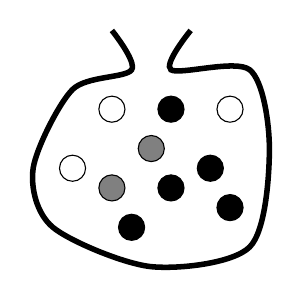
\begin{tikzpicture} 
		\node [fill=white, draw=black, shape=circle] (0) at (-1.25, 0.5) {};
		\node [fill=white, draw=black, shape=circle] (1) at (-0.75, 1.25) {};
		\node [fill=black, draw=black, shape=circle] (2) at (0, 1.25) {};
		\node [fill=gray, draw=black, shape=circle] (3) at (-0.25, 0.75) {};
		\node [fill=gray, draw=black, shape=circle] (4) at (-0.75, 0.25) {};
		\node [fill=black, draw=black, shape=circle] (5) at (0, 0.25) {};
		\node [fill=black, draw=black, shape=circle] (6) at (0.5, 0.5) {};
		\node [fill=black, draw=black, shape=circle] (7) at (0.75, 0) {};
		\node [fill=black, draw=black, shape=circle] (8) at (-0.5, -0.25) {};
		\node [fill=white, draw=black, shape=circle] (9) at (0.75, 1.25) {};
		\draw[ line width=2pt] plot [smooth] coordinates {(-0.75, 2.25)  (-0.5, 1.75)  (-1.25, 1.5) (-1.75, 0.5) (-1.5, -0.25) (-0.25, -0.75) (1, -0.5) (1.25, 0.75)  (1, 1.75)  (0, 1.75)   (0.25, 2.25) }; 
	\end{tikzpicture}	
}
\end{exercise}
\begin{exercise} On fait tourner deux aiguilles et on note le couple de couleurs obtenues.On suppose que les aiguilles s'arrètent au hasard sur les secteurs de même taille. \\ 
\noindent
\parbox[position=t]{0.6\linewidth}{
\begin{enumerate}[label=\arabic*),leftmargin=*]
	\item Complète le diagramme de l'univers de cette expérience : \\
	\renewcommand{\arraystretch}{1.4}
	\begin{tabular}{|*5{c|}}
		\cline{3-5}
		\multicolumn{2}{c|}{\multirow{2}{*}{}} & \multicolumn{3}{c|}{issues équiprobables aiguille \no 2}  \\ \cline{3-5}
		\multicolumn{2}{c|}{}   & Blanc   &      &      \\ \hline
		\multirow{2}{*}{\rotatebox[origin=c]{90}{\parbox{2.2cm}{\small issues   équiprobables   aiguille \no 1}}}	  
		& Noir   & (N~;~B )    &   &    \\ \cline{2-5}
		&    &     & \phantom{(Gris;Blanc)}  &    \\ \cline{2-5}
		&     &   &     & \phantom{(Blanc;Blanc)}  \\  \hline
	\end{tabular} 
\end{enumerate} 
}
\hfill 
\parbox[position=t]{0.36\linewidth}{ \centering
	\noindent
	\hfill
	\begin{tikzpicture}[scale=0.6]
		\tkzSetUpPoint[size=2, fill=black]
		\tkzfctset{tan style/.style={->,>=latex, color=red, line width=1.2pt}}   
		\tkzSetUpLine[line width= 1.2pt, add=.5 and .5]  
		%			\tkzInit[xmin=-1.0,ymin=-1.0,xmax=6.5,ymax=2.8]
		%			\tkzClip
		
		\def\a{2.5}
		\tkzDefPoint(0,0){O} 
		
		\foreach \x [count = \xi] in {0,120,240}
		{
			\tkzDefShiftPoint[O](\x:\a){A\xi}
		} 
		\tkzFillSector[draw,line width=1.2pt,fill=white, ](O,A1)(A2)
		\tkzFillSector[draw,line width=1.2pt,fill=black](O,A2)(A3)
		\tkzFillSector[draw,line width=1.2pt,fill=gray,](O,A3)(A1)  
		
		\tkzDefPoint(1,-0.5){A}
		\tkzDefPoint(-1.5,0.75){B}
		\tkzDrawSegment[line width=1.2pt, |->, >=latex,fill=black, draw=white](A,B) 
	\end{tikzpicture}
	\hfill 
	\begin{tikzpicture}[scale=0.6]
		\tkzSetUpPoint[size=2, fill=black]
		\tkzfctset{tan style/.style={->,>=latex, color=red, line width=1.2pt}}   
		\tkzSetUpLine[line width= 1.2pt, add=.5 and .5]  
		%			\tkzInit[xmin=-1.0,ymin=-1.0,xmax=6.5,ymax=2.8]
		%			\tkzClip
		
		\def\a{2.5}
		\tkzDefPoint(0,0){O} 
		
		\foreach \x [count = \xi] in {0,120,240}
		{
			\tkzDefShiftPoint[O](\x:\a){A\xi}
		} 
		\tkzFillSector[draw,line width=1.2pt,fill=white, ](O,A1)(A2)
		\tkzFillSector[draw,line width=1.2pt,fill=white](O,A2)(A3)
		\tkzFillSector[draw,line width=1.2pt,fill=gray,](O,A3)(A1)  
		
		\tkzDefPoint(-1,-0.5){A}
		\tkzDefPoint(+1.5,0.75){B}
		\tkzDrawSegment[line width=1.2pt, |->, >=latex,fill=black, draw=black](A,B) 
	\end{tikzpicture}
	\hfill\null \\
	\null\hfill
	\textbf{Aiguille \no 1}
	\hfill
	\textbf{Aiguille \no 2}
	\hfill\null
}  
\vspace{0.5em}
\begin{spacing}{1.8}
\begin{enumerate}[label=\arabic*),leftmargin=*,start=2]
	\item $P(\text{\og obtenir deux couleurs identiques\fg})=$\dotfill 
	\item $P(\text{\og obtenir deux couleurs différentes \fg})=$\dotfill 
\end{enumerate}
\end{spacing}\vspace{-1em}
 \end{exercise}
\begin{exercise}  \hfill \\
\noindent 
\parbox{0.45\linewidth}{ 
On lance un jeton et  un dé cubique équilibrés. \\
Compléter le diagramme de l'univers des issues possibles et déterminer : \\
$P(\text{\og obtenir face ou un diviseur de 12\fg})=\dotfill$
}
\hfill  
\parbox[position=t]{0.50\columnwidth}{\centering 
\renewcommand{\arraystretch}{1.4} 
	\begin{tabular}{|*8{c|}}
		\cline{3-8}
		\multicolumn{2}{c|}{\multirow{2}{*}{}} & \multicolumn{6}{c|}{issues équiprobables du dé}  \\ \cline{3-8}
		\multicolumn{2}{c|}{}   &  1 &       &    &    &    &   \\ \hline
		\multirow{2}{*}{\rotatebox[origin=c]{0}{\parbox{2cm}{\small issues   équiprobables   de la pièce}}}	  
		&  Pile  &   P1  &  \phantom{P2}  & \phantom{P3}  & \phantom{P4} & \phantom{P5} & \phantom{P6}  \\ \cline{2-8}
		&     &   &    &   &  &  &  \\  \hline
	\end{tabular}
}  	 
\end{exercise}
\begin{exercise}[paradoxe des bancs] Dans la cours du lycée, il y a trois bancs à deux places. Oto est déjà assis pour prendre son déjeuner. Tasha va s'asseoir au hasard. 
	Quark affirme que la probabilité qu'ils se retrouvent sur le même banc est de $\tfrac{1}{3}$. Nog   pense plutôt que cette probabilité est de $\tfrac{1}{5}$
\begin{enumerate}[label=\arabic*),leftmargin=*,start=1]
	\item Expliquer pourquoi Quark et Nog ont raison !
	\item Surligner les passages des énoncés des exercices précédents qui suggèrent une équiprobabilité.
\end{enumerate}
\end{exercise} 
\begin{exercise} Pour la roue de loterie ci-dessous, le joeur Bleu gagne si l'aiguille s'arrète sur la couleur bleue, et le joueur Jaune gagne si l'aiguille s'arrète sur la couleur jaune.\medskip\\
\noindent
\parbox{0.7\linewidth}{
\begin{enumerate}[label=\arabic*),leftmargin=*,start=1]
	\item Faire tourner l'aiguille distribuée 24 fois, et relever la fréquence obtenue de victoire de chaque joueur. Mettre en commun avec votre binôme et  compléter le tableau de fréquence.\\
	\renewcommand{\arraystretch}{1.5} 
	\begin{tabular}{|c|c|c|c|} 
		\cline{2-4}
		\multicolumn{1}{c|}{\multirow{1}{*}{}}
		   &\textbf{Bleu} & \textbf{Jaune} & \textbf{Total}\\ \hline
		fréquence sur 24 lancers & \rule{0pt}{1.8em} & & \\ \hline
		fréquence du binôme sur 24 lancers & \rule{0pt}{1.8em} & & \\ \hline
		fréquence relative sur 48 lancers & \rule{0pt}{1.8em} & &\\ \hline 
	\end{tabular}
\medskip
	\item Donner une estimation de la probabilité de gagner du joueur Bleu.
	\item Donner une estimation au degré près de la somme des angles au centre des secteurs bleus de la roue.
\end{enumerate} 
}
\hfill 
\parbox{0.33\linewidth}{\centering 
	\begin{tikzpicture}[scale=1.0]
		\tkzSetUpPoint[size=2, fill=black]
		\tkzfctset{tan style/.style={->,>=latex, color=red, line width=1.2pt}}   
		\tkzSetUpLine[line width= 1.2pt, add=.5 and .5]  
		%			\tkzInit[xmin=-1.0,ymin=-1.0,xmax=6.5,ymax=2.8]
		%			\tkzClip
		
		\def\a{2.8}
		\tkzDefPoint(0,0){O} 
		
		\foreach \x [count = \xi] in {0,14.4,72,100.8,144,187.2,230.4,244.8,256.2,302.4,360}
		{
			\tkzDefShiftPoint[O](\x-10:\a){A\xi}
		} 
		\tkzFillSector[draw,line width=1.2pt,color=yellow  ](O,A1)(A2)
		\tkzFillSector[draw,line width=1.2pt,color=blue ](O,A2)(A3)
		\tkzFillSector[draw,line width=1.2pt,color=yellow  ](O,A3)(A4)
		\tkzFillSector[draw,line width=1.2pt,color=blue](O,A4)(A5)
		\tkzFillSector[draw,line width=1.2pt,color=yellow  ](O,A5)(A6)
		\tkzFillSector[draw,line width=1.2pt,color=blue ](O,A6)(A7)
		\tkzFillSector[draw,line width=1.2pt,color=yellow  ](O,A7)(A8)
		\tkzFillSector[draw,line width=1.2pt,color=blue](O,A8)(A9)
		\tkzFillSector[draw,line width=1.2pt,color=yellow ](O,A9)(A10)
		\tkzFillSector[draw,line width=1.2pt,color=blue  ](O,A10)(A11) 
		
		\tkzDefPoint(1,-0.5){A}
		\tkzDefPoint(-1.5,0.75){B}
		\tkzDrawSegment[line width=1.2pt, |->, >=latex](A,B) 
	\end{tikzpicture}  
}  
\end{exercise} 
\medskip
\begin{exercise}[Avec deux dés] 
	On lance simultanément un dé Noir et un dé Bleu (cubiques) et on note la somme $S$ des deux nombres obtenus.  On cherche la loi de probabilité des sommes possibles.
	\begin{enumerate}[label=\arabic*),leftmargin=*]
		\item Complète le tableau à double entrée ci-dessous avec les sommes obtenues.  \\
		\noindent  
		\parbox[position=t]{0.55\columnwidth}{\centering 
			\begin{tabular}{|*8{c|}}
				\cline{3-8}
				\multicolumn{2}{c|}{\multirow{2}{*}{}} & \multicolumn{6}{c|}{Dé \no 2}  \\ \cline{3-8}
				\multicolumn{2}{c|}{}   &  1 &  2   &3  & 4 & 5 & 6 \\ \hline
				\multirow{6}{*}{\rotatebox[origin=c]{90}{Dé \no 1}}	  
				& 1  &  \rule{0em}{1.5em} &   &  & & &  \\ \cline{2-8}
				& 2  & \rule{0pt}{1.5em}\rule{1.8em}{0em}  &  \rule{1.8em}{0em}  &  \rule{1.8em}{0em}&\rule{1.8em}{0em} &\rule{1.8em}{0em} &  \rule{1.8em}{0em}\\ \cline{2-8}
				& 3  & \rule{0pt}{1.5em}  &   &   & & &  \\ \cline{2-8}
				& 4  & \rule{0pt}{1.5em}  &   &  &   & &  \\ \cline{2-8}
				& 5  & \rule{0pt}{1.5em}  &   &  & &   &  \\ \cline{2-8}
				& 6  &  \rule{0pt}{1.5em} &   &  & & &   \\ \hline
			\end{tabular}
		}  \hfill
		\parbox[position=t]{0.45\columnwidth}{  
			\begin{tikzpicture}[xscale=0.5, yscale=1]
				\tkzSetUpPoint[size=4, fill=black]
				\tkzfctset{tan style/.style={->,>=latex, color=red, line width=1.2pt}}  
				\tkzInit[xmin=1,xmax=13,ymin=0,ymax=6,xstep=1.0, ystep=1];
				\begin{scope}[dashed] 
					\tkzGrid[color=gray, line width=0.5pt]
				\end{scope}  
				\tkzDrawX[  noticks, font=\scriptsize, line width=2pt, label=$k$, above  ] 
				\tkzLabelX[font=\scriptsize]
				\tkzDrawY[  noticks,  font=\scriptsize, line width=2pt , label={$P(S=k)$}, right ]  
				\tkzLabelY[ orig=false,frac=36,  font=\scriptsize, text=blue,left = 6pt]
				%	\tkzLabelXY[orig = false,  font=\scriptsize]
				%	\tkzRep[color  = Maroon,line width = 2pt, posxlabel=below, posylabel=left, xnorm=1, ynorm=1]  
			\end{tikzpicture}  
		}
		\item Sachant que les deux dés sont équilibrés, en déduire la loi de probabilité des sommes obtenues
		\begin{table}[H]\centering
			\begin{tabularx}{0.95\linewidth}{|c?*{11}{>{\centering \arraybackslash}X|}c|} \hline
				\rule{0pt}{1.8em} $k$ & 2 &   &   &  &  &&  &&&&& Total \\ \hline
				\rule{0pt}{1.8em}	$P(S=k)$&   &   &   &   & &  &   & &&&&  \\\hline
			\end{tabularx}
		\end{table} 
		\item Représenter dans le graphique ci-dessus la loi de probabilité de la somme.%À vous de préciser l'échelle verticale. 
		\item Déterminer les probabilités des événements suivants (ÉCRIRE CLAIREMENT $P(\ldots)=\ldots$):
		%	\begin{multicols}{2}
			\vspace{-0.5em} 
		\begin{multicols}{2}
		\begin{spacing}{1.8}
			\begin{enumerate}[label={$\Alph*=$},leftmargin=*]
				\item \og somme égale à 4 \fg\dotfill 
				\item \og somme égale à 12 \dotfill
				\item \og somme supérieure ou égale à 7 \fg\dotfill
				\item \og somme strictement inférieure à 4 \fg\dotfill
				\item \og somme paire \fg\dotfill
				\item \og somme égale à 7 et produit égal à 12 \fg\dotfill
			\end{enumerate}  
		\end{spacing}
	\end{multicols}
	\vspace{-1em} 
			%\end{multicols}
		\end{enumerate}  
	\end{exercise} 
\begin{exercise} \label{chapter09:exercice:SumDice}
	Détermine et représente la loi de la somme des faces pour les dés distribués. On supposera que les dés sont équilibrés, et on choisira les échelles adaptées. \hfill \\
	\noindent  
	\parbox[position=t]{0.55\columnwidth}{\centering 
		\begin{tabular}{|*8{c|}}
			\cline{3-8}
			\multicolumn{2}{c|}{\multirow{2}{*}{}} & \multicolumn{6}{c|}{Dé \no 2}  \\ \cline{3-8}
			\multicolumn{2}{c|}{}   &  \rule{0em}{1.5em}  &      &   &   &   &   \\ \hline
			\multirow{6}{*}{\rotatebox[origin=c]{90}{Dé \no 1}}	  
			&    &   \rule{0em}{1.5em} &   &  & & &  \\ \cline{2-8}
			& \rule{1.8em}{0em}   & \rule{0pt}{1.5em}\rule{1.8em}{0em}  &  \rule{1.8em}{0em}  &  \rule{1.8em}{0em}&\rule{1.8em}{0em} &\rule{1.8em}{0em} &  \rule{1.8em}{0em}\\ \cline{2-8}
			&    & \rule{0pt}{1.5em}  &   &   & & &  \\ \cline{2-8}
			&    & \rule{0pt}{1.5em}  &   &  &   & &  \\ \cline{2-8}
			&    & \rule{0pt}{1.5em}  &   &  & &   &  \\ \cline{2-8}
			&    &  \rule{0pt}{1.5em} &   &  & & &   \\ \hline
		\end{tabular}
	}  \hfill
	\parbox[position=t]{0.45\columnwidth}{  
		\begin{tikzpicture}[xscale=0.5, yscale=0.5]
			\tkzSetUpPoint[size=4, fill=black]
			\tkzfctset{tan style/.style={->,>=latex, color=red, line width=1.2pt}}  
			\tkzInit[xmin=0,xmax=14,ymin=0,ymax=12,xstep=1.0, ystep=1];
			\begin{scope}[dashed] 
				\tkzGrid[color=gray, line width=0.5pt]
			\end{scope}  
			\tkzDrawX[  noticks, font=\scriptsize, line width=2pt, label=$k$, above  ] 
			%		\tkzLabelX[font=\scriptsize]
			\tkzDrawY[  noticks,  font=\scriptsize, line width=2pt , label={$P(S=k)$}, right ]  
			%	\tkzLabelXY[orig = false,  font=\scriptsize]
			%	\tkzRep[color  = Maroon,line width = 2pt, posxlabel=below, posylabel=left, xnorm=1, ynorm=1]  
		\end{tikzpicture}  
	} 
\\
%	\begin{table}[H]\centering
		\begin{tabularx}{0.95\linewidth}{|c?*{11}{>{\centering \arraybackslash}X|}c|} \hline
			\rule{0pt}{1.8em} $k$ &   &   &   &  &  &&  &&&&& Total \\ \hline
			\rule{0pt}{1.8em}	$P(S=k)$&   &   &   &   & &  &   & &&&&  \\\hline
		\end{tabularx}
%	\end{table}  
\\
	\noindent  
	\parbox[position=t]{0.55\columnwidth}{\centering 
		\begin{tabular}{|*8{c|}}
			\cline{3-8}
			\multicolumn{2}{c|}{\multirow{2}{*}{}} & \multicolumn{6}{c|}{Dé \no 2}  \\ \cline{3-8}
			\multicolumn{2}{c|}{}   &  \rule{0em}{1.5em}  &      &   &   &   &   \\ \hline
			\multirow{6}{*}{\rotatebox[origin=c]{90}{Dé \no 1}}	  
			&    &   \rule{0em}{1.5em} &   &  & & &  \\ \cline{2-8}
			& \rule{1.8em}{0em}   & \rule{0pt}{1.5em}\rule{1.8em}{0em}  &  \rule{1.8em}{0em}  &  \rule{1.8em}{0em}&\rule{1.8em}{0em} &\rule{1.8em}{0em} &  \rule{1.8em}{0em}\\ \cline{2-8}
			&    & \rule{0pt}{1.5em}  &   &   & & &  \\ \cline{2-8}
			&    & \rule{0pt}{1.5em}  &   &  &   & &  \\ \cline{2-8}
			&    & \rule{0pt}{1.5em}  &   &  & &   &  \\ \cline{2-8}
			&    &  \rule{0pt}{1.5em} &   &  & & &   \\ \hline
		\end{tabular}
	}  \hfill
	\parbox[position=t]{0.45\columnwidth}{  
		\begin{tikzpicture}[xscale=0.5, yscale=0.5]
			\tkzSetUpPoint[size=4, fill=black]
			\tkzfctset{tan style/.style={->,>=latex, color=red, line width=1.2pt}}  
			\tkzInit[xmin=0,xmax=14,ymin=0,ymax=12,xstep=1.0, ystep=1];
			\begin{scope}[dashed] 
				\tkzGrid[color=gray, line width=0.5pt]
			\end{scope}  
			\tkzDrawX[  noticks, font=\scriptsize, line width=2pt, label=$k$, above  ] 
			%		\tkzLabelX[font=\scriptsize]
			\tkzDrawY[  noticks,  font=\scriptsize, line width=2pt , label={$P(S=k)$}, right ]  
			%	\tkzLabelXY[orig = false,  font=\scriptsize]
			%	\tkzRep[color  = Maroon,line width = 2pt, posxlabel=below, posylabel=left, xnorm=1, ynorm=1]  
		\end{tikzpicture}  
	} 
\\
%	\begin{table}[H]\centering
		\begin{tabularx}{0.95\linewidth}{|c?*{11}{>{\centering \arraybackslash}X|}c|} \hline
			\rule{0pt}{1.8em} $k$ &   &   &   &  &  &&  &&&&& Total \\ \hline
			\rule{0pt}{1.8em}	$P(S=k)$&   &   &   &   & &  &   & &&&&  \\\hline
		\end{tabularx}
%	\end{table} 
\\
	\noindent  
\parbox[position=t]{0.55\columnwidth}{\centering 
	\begin{tabular}{|*8{c|}}
		\cline{3-8}
		\multicolumn{2}{c|}{\multirow{2}{*}{}} & \multicolumn{6}{c|}{Dé \no 2}  \\ \cline{3-8}
		\multicolumn{2}{c|}{}   &  \rule{0em}{1.5em}  &      &   &   &   &   \\ \hline
		\multirow{6}{*}{\rotatebox[origin=c]{90}{Dé \no 1}}	  
		&    &   \rule{0em}{1.5em} &   &  & & &  \\ \cline{2-8}
		& \rule{1.8em}{0em}   & \rule{0pt}{1.5em}\rule{1.8em}{0em}  &  \rule{1.8em}{0em}  &  \rule{1.8em}{0em}&\rule{1.8em}{0em} &\rule{1.8em}{0em} &  \rule{1.8em}{0em}\\ \cline{2-8}
		&    & \rule{0pt}{1.5em}  &   &   & & &  \\ \cline{2-8}
		&    & \rule{0pt}{1.5em}  &   &  &   & &  \\ \cline{2-8}
		&    & \rule{0pt}{1.5em}  &   &  & &   &  \\ \cline{2-8}
		&    &  \rule{0pt}{1.5em} &   &  & & &   \\ \hline
	\end{tabular}
}  \hfill
\parbox[position=t]{0.45\columnwidth}{  
	\begin{tikzpicture}[xscale=0.5, yscale=0.5]
		\tkzSetUpPoint[size=4, fill=black]
		\tkzfctset{tan style/.style={->,>=latex, color=red, line width=1.2pt}}  
		\tkzInit[xmin=0,xmax=14,ymin=0,ymax=12,xstep=1.0, ystep=1];
		\begin{scope}[dashed] 
			\tkzGrid[color=gray, line width=0.5pt]
		\end{scope}  
		\tkzDrawX[  noticks, font=\scriptsize, line width=2pt, label=$k$, above  ] 
		%		\tkzLabelX[font=\scriptsize]
		\tkzDrawY[  noticks,  font=\scriptsize, line width=2pt , label={$P(S=k)$}, right ]  
		%	\tkzLabelXY[orig = false,  font=\scriptsize]
		%	\tkzRep[color  = Maroon,line width = 2pt, posxlabel=below, posylabel=left, xnorm=1, ynorm=1]  
	\end{tikzpicture}  
} 
\end{exercise}


%----------------------------------------------------------------------------------------
%	 
%----------------------------------------------------------------------------------------
\newpage 
\begin{example}[modéliser avec des diagrammes de Venn ou des tableaux croisés des effectifs] \hfill \\
\noindent 
\parbox{0.35\linewidth}{
Sur 60 élèves d'un lycée :
\begin{enumerate}[label=\textbullet,leftmargin=*]
		\item 8 font club Théatre et  Musique
		\item 6 font club Théatre mais pas Musique.
		\item 19 font le club Musique.
	\end{enumerate} 
\begin{enumerate}[label=\arabic*),leftmargin=*,start=1]
	\item Compléter le tableau croisé des effectifs et le diagramme de Venn  
\end{enumerate} 
}\hfill
	\parbox{0.30\linewidth}{ \centering   
	\begin{venndiagram2sets}[tikzoptions={scale=1.0,thick},
		tikzoptions={text opacity=1,fill opacity=0.25},
		labelA={},
		labelB={}, 
		labelOnlyA={$\ldots$},
		labelOnlyB={$\ldots$}, 
		labelAB={$8$},  
		labelNotAB={$\ldots$} ]
		\setpostvennhook
		{
			\draw[<-] (labelA) -- ++(135:1.5cm) node[above] {$T$};
			\draw[<-] (labelB) -- ++(45:1.5cm) node[above] {$M$};  
			\draw (venn bottom left) -- (venn bottom right) node[midway, below ]{$\operatorname{Card}(\Omega)=60$}; 
		}
	\end{venndiagram2sets} 
}
\parbox{0.30\linewidth}{ \centering   
\begin{tabular}{|*4{c|}}
	\cline{2-4} 
	\multicolumn{1}{c|}{\rule{0pt}{1.8em}\rule{2em}{0em}}   & $T$ &  $\overline{T}$ & \textbf{Total} \\ \hline
	\rule{0pt}{1.8em}	$M$			 &   \textbf{8}   & 	 &     \\ \cline{1-4}
	\rule{0pt}{1.8em} $\overline{M}$ &   \rule{2.2em}{0em} 	&   \rule{2.2em}{0em}   & \rule{2.2em}{0em}  \\ \hline  
	\multicolumn{1}{|c|}{\textbf{\rule{0pt}{1.8em}Total}} &    &    &  \textbf{60} \\\hline
\end{tabular}   
}
\begin{enumerate}[label=\arabic*),leftmargin=*,start=2]
%	\item Compléter le tableau double entrée et le diagramme de Venn 
	\item 		On choisit un élève au hasard parmi ceux du lycée. \\
	Déterminer la probabilité que l'élève choisi ne fasse partie d'aucun club :\hfill 
	$P(\overline{M}\cap\overline{T})=\frac{\phantom{35}}{60}$\hfill\null
\end{enumerate}  
\end{example} 
\begin{exercise} Sur 85 personnes interrogées sur leur préférences entre café et thé :  18 n'aiment aucune des boissons, 29 aiment le thé mais pas le café et 22 aiment le café, mais pas le thé.\\
	Soit les événements : 
	$C=$\og l'individu aime le café\fg et 
	$T=$ \og  l'individu aime le thé\fg.\hfill \\
	\noindent
	\parbox{0.4\linewidth}{  
		\begin{enumerate}[label=\arabic*), leftmargin=*] 
			\item Compléter le tableau effectifs croisés et le diagramme de Venn
			\item On choisit un individu au hasard. Donner la probabilité qu'il aime le café et le thé.
		\end{enumerate} 	
	}\hfill 
	\parbox{0.3\linewidth}{\centering
		\begin{venndiagram2sets}[tikzoptions={scale=0.95,thick},
			tikzoptions={text opacity=1,fill opacity=0.25},
			labelA={},
			labelB={}, 
			labelOnlyA={$\ldots$},
			labelOnlyB={$\ldots$}, 
			labelAB={$\ldots$},  
			labelNotAB={$\ldots$} ]
			\setpostvennhook
			{
				\draw[<-] (labelA) -- ++(135:1.3cm) node[above] {Thé};
				\draw[<-] (labelB) -- ++(45:1.3cm) node[above] {Café};  
				\draw (venn bottom left) -- (venn bottom right) node[midway, below ]{$\operatorname{Card}(\Omega)=\ldots$}; 
			}
		\end{venndiagram2sets} 
	}\hfill
	\parbox{0.25\linewidth}{\centering
		\begin{tabular}{|*4{c|}}
			\cline{2-4} 
			\multicolumn{1}{c|}{\rule{0pt}{1.8em}\rule{2em}{0em}}   & $T$ &  $\overline{T}$ & \textbf{Total} \\ \hline
			\rule{0pt}{1.8em}	$C$			 &      & 	$\qquad$ &     \\ \cline{1-4}
			\rule{0pt}{1.8em} $\overline{C}$ &   $\qquad$	&  $\qquad$  &  \rule{2.2em}{0em} \\ \hline  
			\multicolumn{1}{|c|}{\textbf{\rule{0pt}{1.8em}Total}} & \rule{2.0em}{0em}    &    \rule{2.0em}{0em}  &  85 \\\hline
		\end{tabular}  
	} 
	
\end{exercise}

\begin{exercise} 
	Afin de mieux connaître sa clientèle, une station de sports d'hiver a 
	effectué une enquête auprès de 250~skieurs. 
	Voici la synthèse des réponses au sondage:
	\begin{enumerate}[label=\textbullet, leftmargin=*]
		\item deux tiers des personnes qui viennent tous les week-ends possèdent 
		leur matériel;
		\item  la moitié des personnes venant deux semaines par an possèdent 
		également leur matériel;
		\item   44\% des personnes interrogées louent sur place.
	\end{enumerate} 
	\noindent\parbox{0.6\linewidth}{ 
	On considère les événements suivants.
\begin{enumerate}[label=\textbullet,leftmargin=*]
			\item $M$: \og la personne possède son matériel \fg;
			\item $L:$ \og la personne loue ses skis sur place \fg; 
			\item $A:$ \og la personne loue ses skis ailleurs \fg; 
			\item $S:$ \og la personne vient une semaine par an \fg;
			\item $W:$ \og la personne vient tous les week-ends \fg;
			\item $Q:$ \og la personne vient deux semaines par an \fg.
	\end{enumerate}
	}\hfill 
	\parbox{0.4\linewidth}{
		\renewcommand{\arraystretch}{1.5} 
		\begin{tabular}{|c|c|c|c|c|c|c|}
			\hline
			& M & L & A & Total \\\hline
			S & 25 &  &  & \rule{1.8em}{0pt} \\\hline
			W &  &  & 5 & 30 \\\hline
			Q &  & 30 &  & 100 \\\hline
			Total & \rule{1.8em}{0pt} &\rule{1.8em}{0pt}  &  \rule{1.8em}{0pt}& 250\\\hline
		\end{tabular}
	}
	\begin{enumerate}[label=\arabic*), leftmargin=*] 
		\item Compléter le tableau ci-contre présentant la synthèse des réponses.
		\item On choisit au hasard un client parmi les 250 personnes.  Déterminer les probabilités :
		\vspace{-0.5em}
		\begin{spacing}{2}
		\begin{enumerate}[label={},leftmargin=*]
			\item   $P(Q)=$\dotfill    $P(L)=$\dotfill
			   $P(\overline{M})=$\dotfill 
			   \item	$P(Q\cap L)=$\dotfill 
			  $P(Q\cup L)=$\dotfill  $P(\overline{Q}\cap L)=$\dotfill
		\end{enumerate}  
		\end{spacing}
	\vspace{-1em} 
	\end{enumerate}
\end{exercise}

%----------------------------------------------------------------------------------------
%	 
%----------------------------------------------------------------------------------------
\newpage 
\begin{exercise} Sur 100 personnes interrogées :  23 affirment posséder un chat, 31 affirment posséder un chien et 56 affirment posséder ni chat ni chien. 
	\hfill \\
	\noindent
	\parbox{0.4\linewidth}{  
		Soit les événements : 
		$C=$\og l'individu a un chat\fg et 
		$D=$ \og  l'individu a un chien\fg.
		\begin{enumerate}[label=\arabic*), leftmargin=*] 
			\item Compléter le diagramme de Venn et le tableau croisé des effectifs.
			\item On choisit un individu au hasard. Donner la probabilité qu'il a un chien et un chat ?
		\end{enumerate} 	
	}\hfill 
	\parbox{0.3\linewidth}{\centering
		\begin{venndiagram2sets}[tikzoptions={scale=0.95,thick},
			tikzoptions={text opacity=1,fill opacity=0.25},
			labelA={},
			labelB={}, 
			labelOnlyA={$\ldots$},
			labelOnlyB={$\ldots$}, 
			labelAB={$\ldots$},  
			labelNotAB={$\ldots$} ]
			\setpostvennhook
			{
				\draw[<-] (labelA) -- ++(135:1.3cm) node[above] {C};
				\draw[<-] (labelB) -- ++(45:1.3cm) node[above] {D};  
				\draw (venn bottom left) -- (venn bottom right) node[midway, below ]{$\operatorname{Card}(\Omega)=\ldots$}; 
			}
		\end{venndiagram2sets} 
	}\hfill
	\parbox{0.25\linewidth}{\centering
		\begin{tabular}{|*4{c|}}
			\cline{2-4} 
			\multicolumn{1}{c|}{\rule{0pt}{1.8em}\rule{2em}{0em}}   & $D$ &  $\overline{D}$ & \textbf{Total} \\ \hline
			\rule{0pt}{1.8em}	$C$			 &      & 	$\qquad$ &     \\ \cline{1-4}
			\rule{0pt}{1.8em} $\overline{C}$ &   $\qquad$	&  $\qquad$  &  \rule{2.2em}{0em} \\ \hline  
			\multicolumn{1}{|c|}{\textbf{\rule{0pt}{1.8em}Total}} & \rule{2.0em}{0em}    &    \rule{2.0em}{0em}  &    \\\hline
		\end{tabular}  
	} 
	
\end{exercise}

\begin{exercise} \hfill 
	\\
	\begin{minipage}{0.65\columnwidth} 
		Dans un établissement scolaire, on a interrogé 480 élèves de Seconde sur leur
séjour en Espagne, en Italie et en Allemagne :
		\begin{description}
			\item[$\bullet$]   220 élèves ont séjourné en Allemagne ;
			\item[$\bullet$] 218 élèves en Italie et 217 en Espagne ;
			\item[$\bullet$]  105 ont séjourné en Italie et en Espagne ;
			\item[$\bullet$]  100 ont séjourné en Italie et en Allemagne
			\item[$\bullet$]  93 ont séjourné en Espagne et en Allemagne ;
			\item[$\bullet$]  60 élèves n’ont séjourné dans aucun des 3 pays.
		\end{description} 
		\begin{enumerate}[label=\arabic*), leftmargin=*] 
			\item 	Compléter le diagramme de Venn.
			\item On interrroge au hasard un élève. Quelle est la probabilité qu'il a séjourné dans les 3 pays ?
		\end{enumerate}
	\end{minipage}
	\begin{minipage}{0.35\columnwidth} \centering
		\begin{venndiagram3sets}[tikzoptions={scale=1.2,thick},
			tikzoptions={text opacity=1,fill opacity=0.25},
			labelA={},
			labelB={},
			labelC={},
			labelOnlyA={$\ldots$},
			labelOnlyB={$\ldots$},
			labelOnlyC={$\ldots$},
			labelOnlyAB={$\ldots$},
			labelOnlyAC={$\ldots$},
			labelOnlyBC={$\ldots$},
			labelABC={$\ldots$},
			labelNotABC={60} ]
			\setpostvennhook
			{
				\draw[<-] (labelA) -- ++(135:1.5cm) node[above] {Allemagne};
				\draw[<-] (labelB) -- ++(45:1.5cm) node[above] {Espagne}; 
				\draw[<-]  (labelC)  -- ++(-45:1.5cm) node[right] {Italie}; 
				\draw (venn bottom left) -- (venn bottom right) node[midway, below ]{$\abs{\Omega}=480$}; 
			}
		\end{venndiagram3sets} 
	\end{minipage}	 
\end{exercise}
\begin{eBox}
C'est à vous de décider si l'expérience aléatoire est modélisable par un tableau croisé des effectifs ou diagramme de Venn
\end{eBox}
\vspace{-0.5em}
\begin{exercise}\label{chapitre09.ex.dopage} 
	Un nouveau test antidopage est testé sur 36 athlètes. Voici les résultats.
	\begin{enumerate}[label={\textbullet},leftmargin=*]
		\item Il y a 9 athlètes dopés et 6 testés positifs.
		\item 13 athlètes sont soit dopés soit testés positifs.
	\end{enumerate}
	On considère les événements $D=$\og l'athlète est dopé \fg{} et $T^+=$\og l'athlète est testé positif \fg{}. 
Définir par une phrase les événements $D\cap \overline{T^+}$ (Faux négatif) et $\overline{D}\cap T^+$ (Faux positif) et déterminer leur probabilités.  
\end{exercise} 
\begin{exercise}[Des groupes de spécialité]\label{evaluation:probabilite:exercice:01} 
	
	\medskip 
	
	\noindent Dans une classe de 2\up{nde}, il y a 35 élèves :
	\begin{enumerate}[label={\textbullet},leftmargin=*]
		\item 19 ont pris l'enseignement d'exploration \og Méthodes et pratiques scientifiques\fg{}, les autres ont pris l'enseignement d'exploration \og Littérature et société \fg{} ;
		\item il y a 15 garçons ;
		\item 12 filles ont pris l'enseignement d'exploration \og Méthodes et pratiques scientifiques\fg{}.
	\end{enumerate}
	
	\noindent On choisit un élève au hasard dans la classe, chaque élève ayant la même probabilité d'être choisi,
	et on définit les évènements suivants :
	\begin{enumerate}[label={\textbullet},leftmargin=*]
		\item $M$ : l'élève choisi a pris l'enseignement d'exploration \og Méthodes et pratiques scientifiques\fg{} ;
		\item $G$ : l'élève choisi est un garçon.
	\end{enumerate}
	
	\begin{enumerate}[label={\arabic*)},leftmargin=*]
		\item Déterminer les probabilités des  évènements $M$ et $G$.
		\item Définir par une phrase les évènements $M\cap G$, $M \cup G$ et   $\overline{M} \cap G$ et déterminer leurs probabilités.
	\end{enumerate}
	
\end{exercise}

%----------------------------------------------------------------------------------------
%	 
%----------------------------------------------------------------------------------------
\newpage 
\begin{example}[Modéliser à l'aide d'un arbre de probabilité] \hfill \\
Une boite opaque contient 2 rubans rouges et 3 rubans bleus.  On tire au hasard  1 premier ruban de la boite sans regarder (et sans le remettre), puis un second, et on note les couleurs de chaque. \\
On compte  4 issues possibles (non équiprobbles ! il y a plus de rubans bleus que de rouges !) 
\vspace{-0.5em}
\begin{multicols}{2}
\begin{enumerate}[label=\textbullet,leftmargin=* ] 
	\item $BB=$  \og tirer   deux rubans bleus\fg
	\item $RR=$   \og tirer   deux rubans rouges\fg
	\item $BR=$  \og tirer   un ruban bleu puis un ruban rouge \fg
	\item $RB=$   \og tirer   un ruban rouge puis un ruban bleu \fg
\end{enumerate}
\end{multicols}
\vspace{-0.5em} 
		\noindent\parbox[position=b]{0.38\linewidth}{
			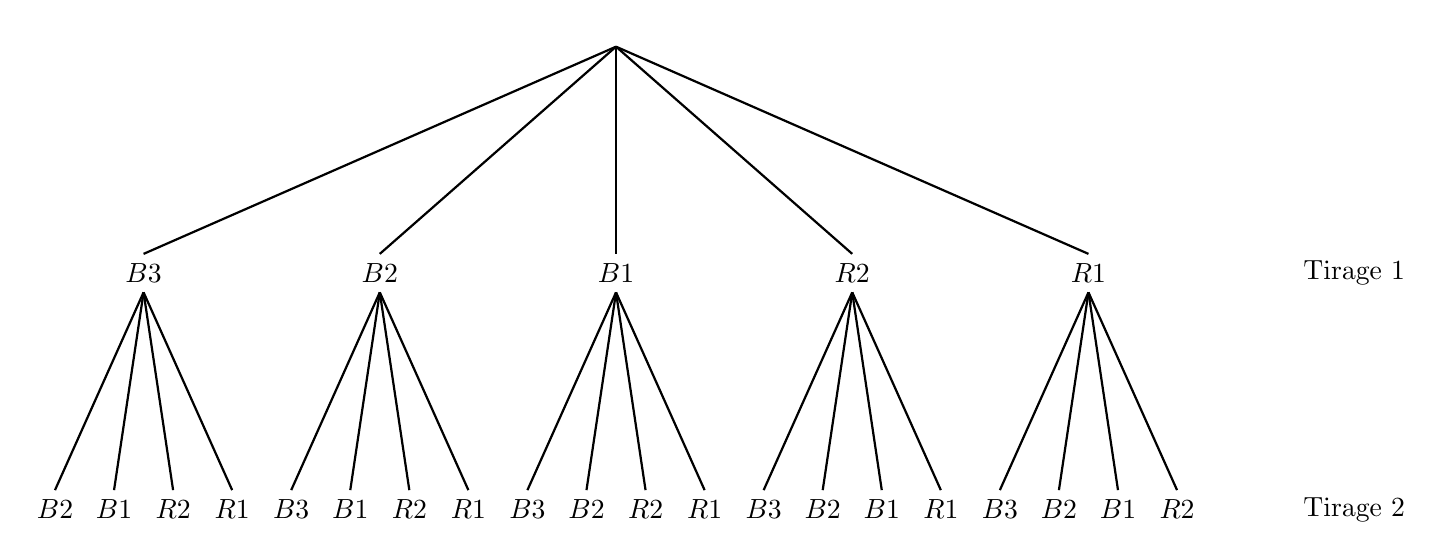
\begin{tikzpicture}[xscale=1,yscale=1]
				
				\def \alpha{-90}
				\def \beta{0}
				\def \xnorm{1.0};
				\def \ynorm{1.0}; 
				\pgftransformcm{\xnorm*cos(\alpha)}{\xnorm*sin(\alpha)}{\ynorm*cos(\beta)}{\ynorm*sin(\beta)}{\pgfpointorigin}
				% Styles (MODIFIABLES)
				\tikzstyle{fleche}=[-,>=latex,thick]
				\tikzstyle{noeud}=[rounded corners=5pt]
				\tikzstyle{feuille}=[]
				\tikzstyle{commentaire}=[black]
				% Dimensions (MODIFIABLES)
				\def\DistanceInterNiveaux{3}
				\def\DistanceInterFeuilles{1.5}
				% Dimensions calculées (NON MODIFIABLES)
				\def\NiveauA{(0.0)*\DistanceInterNiveaux}
				\def\NiveauB{(1.0)*\DistanceInterNiveaux}
				\def\NiveauC{(2.0)*\DistanceInterNiveaux}
				\def\NiveauD{(3.0)*\DistanceInterNiveaux}
				\def\NiveauE{(3.5)*\DistanceInterNiveaux}
				\def\InterFeuilles{(-1)*\DistanceInterFeuilles}
				% Noeuds (MODIFIABLES : Styles et Coefficients d'InterFeuilles)
				\node[commentaire] (epreuve1) at ({\NiveauB},{(-1)*\InterFeuilles}) {Tirage \no 1};
				\node[commentaire] (epreuve2) at ({\NiveauC},{(-1)*\InterFeuilles}) {Tirage \no 2}; 
				%	\node[commentaire] (issues) at ({\NiveauD},{(0)*\InterFeuilles}) {Issues};
				%	\node[commentaire] (probas) at ({\NiveauE},{(0)*\InterFeuilles}) {Probabilités};
				% 
				\node[noeud] (R) at ({\NiveauA},{(5.25)*\InterFeuilles}) {};
				\node[noeud] (Ra) at ({\NiveauB},{(1.25)*\InterFeuilles}) {$R1$};
				\node[feuille] (Raa) at ({\NiveauC},{(0.5)*\InterFeuilles}) {$R2$}; 
				\node[feuille] (Rab) at ({\NiveauC},{(1)*\InterFeuilles}) {$B1$}; 
				\node[feuille] (Rac) at ({\NiveauC},{(1.5)*\InterFeuilles}) {$B2$}; 
				\node[feuille] (Rad) at ({\NiveauC},{(2)*\InterFeuilles}) {$B3$}; 
%				\node[feuille] (Rae) at ({\NiveauC},{(2.5)*\InterFeuilles}) {$B4$}; 
				\node[noeud] (Rb) at ({\NiveauB},{(3.25)*\InterFeuilles}) {$R2$};
				\node[feuille] (Rba) at ({\NiveauC},{(2.5)*\InterFeuilles}) {$R1$}; 
				\node[feuille] (Rbb) at ({\NiveauC},{(3.0)*\InterFeuilles}) {$B1$}; 
				\node[feuille] (Rbc) at ({\NiveauC},{(3.5)*\InterFeuilles}) {$B2$}; 
				\node[feuille] (Rbd) at ({\NiveauC},{(4.0)*\InterFeuilles}) {$B3$}; 
%				\node[feuille] (Rbe) at ({\NiveauC},{(5.0)*\InterFeuilles}) {$B4$};  
				\node[noeud] (Rc) at ({\NiveauB},{(5.25)*\InterFeuilles}) {$B1$}; 
				\node[feuille] (Rca) at ({\NiveauC},{(4.5)*\InterFeuilles}) {$R1$}; 
				\node[feuille] (Rcb) at ({\NiveauC},{(5.0)*\InterFeuilles}) {$R2$}; 
				\node[feuille] (Rcc) at ({\NiveauC},{(5.5)*\InterFeuilles}) {$B2$}; 
				\node[feuille] (Rcd) at ({\NiveauC},{(6.0)*\InterFeuilles}) {$B3$}; 
				\node[noeud] (Rd) at ({\NiveauB},{(7.25)*\InterFeuilles}) {$B2$}; 
				\node[feuille] (Rda) at ({\NiveauC},{(6.5)*\InterFeuilles}) {$R1$}; 
				\node[feuille] (Rdb) at ({\NiveauC},{(7.0)*\InterFeuilles}) {$R2$}; 
				\node[feuille] (Rdc) at ({\NiveauC},{(7.5)*\InterFeuilles}) {$B1$}; 
				\node[feuille] (Rdd) at ({\NiveauC},{(8.0)*\InterFeuilles}) {$B3$}; 
				\node[noeud] (Re) at ({\NiveauB},{(9.25)*\InterFeuilles}) {$B3$}; 
				\node[feuille] (Rea) at ({\NiveauC},{(8.5)*\InterFeuilles}) {$R1$}; 
				\node[feuille] (Reb) at ({\NiveauC},{(9.0)*\InterFeuilles}) {$R2$}; 
				\node[feuille] (Rec) at ({\NiveauC},{(9.5)*\InterFeuilles}) {$B1$}; 
				\node[feuille] (Red) at ({\NiveauC},{(10.0)*\InterFeuilles}) {$B2$};
%				\node[noeud] (Rf) at ({\NiveauB},{(14.0)*\InterFeuilles}) {$B4$};
				%
				%	\node[commentaire] (I1) at ({\NiveauD},{(0.5)*\InterFeuilles}) {$\ldots$}; 
				%	\node[commentaire] (I2) at ({\NiveauD},{(1.0)*\InterFeuilles}) {$\ldots$}; 
				%	\node[commentaire] (I3) at ({\NiveauD},{(1.5)*\InterFeuilles}) {$\ldots$}; 
				%	\node[commentaire] (I4) at ({\NiveauD},{(2.0)*\InterFeuilles}) {$\ldots$};
				% 
				% Arcs (MODIFIABLES : Styles)
				\draw[fleche] (R.south)--(Ra.north) node[midway, above,sloped]{ };
				\draw[fleche] (Ra.south)--(Raa.north) node[midway, above,sloped]{ };
				\draw[fleche] (Ra.south)--(Rab.north) node[midway, below,sloped]{ };
				\draw[fleche] (Ra.south)--(Rac.north) node[midway, below,sloped]{ };
				\draw[fleche] (Ra.south)--(Rad.north) node[midway, below,sloped]{};
%				\draw[fleche] (Ra.east)--(Rae.west) node[midway, below,sloped]{};
				\draw[fleche] (R.south)--(Rb.north) node[midway, below,sloped]{};
				\draw[fleche] (Rb.south)--(Rba.north) node[midway, above,sloped]{};
				\draw[fleche] (Rb.south)--(Rbb.north) node[midway, below,sloped]{};
				\draw[fleche] (Rb.south)--(Rbc.north) node[midway, below,sloped]{};
				\draw[fleche] (Rb.south)--(Rbd.north) node[midway, below,sloped]{};
%				\draw[fleche] (Rb.east)--(Rbe.west) node[midway, below,sloped]{};
				\draw[fleche] (R.south)--(Rc.north) node[midway, below,sloped]{};
				\draw[fleche] (Rc.south)--(Rca.north) node[midway, above,sloped]{};
				\draw[fleche] (Rc.south)--(Rcb.north) node[midway, below,sloped]{};
				\draw[fleche] (Rc.south)--(Rcc.north) node[midway, below,sloped]{};
				\draw[fleche] (Rc.south)--(Rcd.north) node[midway, below,sloped]{};
				\draw[fleche] (R.south)--(Rd.north) node[midway, below,sloped]{};
				\draw[fleche] (Rd.south)--(Rda.north) node[midway, above,sloped]{};
				\draw[fleche] (Rd.south)--(Rdb.north) node[midway, below,sloped]{};
				\draw[fleche] (Rd.south)--(Rdc.north) node[midway, below,sloped]{};
				\draw[fleche] (Rd.south)--(Rdd.north) node[midway, below,sloped]{};
				\draw[fleche] (R.south)--(Re.north) node[midway, below,sloped]{};
				\draw[fleche] (Re.south)--(Rea.north) node[midway, above,sloped]{};
				\draw[fleche] (Re.south)--(Reb.north) node[midway, below,sloped]{};
				\draw[fleche] (Re.south)--(Rec.north) node[midway, below,sloped]{};
				\draw[fleche] (Re.south)--(Red.north) node[midway, below,sloped]{};
%				\draw[fleche] (R.east)--(Rf.west) node[midway, below,sloped]{};
			\end{tikzpicture} 
		}\hfill
\begin{enumerate}[label={\textbullet},leftmargin=*] 
	\item L'expérience aléatoire est constituée de 2 expériences aléatoires élémentaires (1\ier tirage ...).
	\item Chaque niveau correspond à une expérience aléatoire élémentaire.
	\item Les bifurcations à chaque niveau correspondent aux issues possibles d'une l'expérience élémentaire.
	\item Chaque chemin le long de l'arbre correspond à une issue. Le chemin $R1B3$ correspond à l'issue \og $R1$ au tirage \no 1 PUIS $B3$ au tirage \no 2\fg.
	\item Les chemins différents sont des issues incompatibles.
	\item Les issues sont \textbf{équiprobables si le nombre de bifurcations à chaque niveau est le même pour tous les noeuds}. Ici $\tfrac{1}{20}$.
\end{enumerate}	 
\begin{spacing}{1.8}
\begin{enumerate}[label={},leftmargin=* ] 
	\item  $P(RR)= P(R1R2) + P(R2R1)=\frac{2}{20}$, 
	\item $P(BR)= P(\{R1B1,R2B1,R1B2,R2B2,R1B3,R2B3\})=\frac{6}{20}$. 
	\item $P(RB)= \dotfill $.
	\item $P(BB)= \dotfill $.
	\item $P(\text{un ruban rouge est tiré au premier tirage})=\dotfill$
	\item $P(\text{un ruban rouge est tiré au second tirage})=\dotfill$
\end{enumerate}
\end{spacing}
\vspace{-1.0em}
\end{example}
\begin{exercise} On reprend l'exercice précédent avec une boite opaque contenant 2 rubans rouges, 3 rubans bleus, mais cette fois on remmet dans la boite le premier ruban tiré. 
	\vspace{-0.5em}
	\begin{spacing}{1.8}
\begin{enumerate}[label=\arabic*), leftmargin=*]
	\item Comment est modifié l'arbre précédent ? Rajouter en rouge les branches supplémentaires.
	\item Déduire la nouvelle valeur de $P(RR)=\dotfill$
	\item Quelle est la probabilité de tirer aucun ruban rouge ?\dotfill 
	\item $P(\text{un ruban rouge est tiré au second tirage})=\dotfill$
\end{enumerate}
\end{spacing}
\vspace{-1.0em}
\end{exercise} 
%----------------------------------------------------------------------------------------
%	 
%----------------------------------------------------------------------------------------
\newpage 
\begin{exercise}[le menu] 
	Au restaurant scolaire le menu se compose forcement d'une entrée, d'un plat et d'un dessert. Les élèves doivent choisir une entrée parmi Artichaut (A) ou Betterave (B),  puis choisir un plat parmi    Cheval (C), Daube (D) ou Escalope (E)  et choisir un dessert parmi Fromage (F) ou Gâteau (G). 
	\begin{enumerate}[label=\arabic*),leftmargin=*]
		\item Compléter l'arbre et identifier tous menus possibles.\\ 
	\begin{minipage}{1\columnwidth}  
	% Racine à Gauche, développement vers la droite
	\begin{tikzpicture}[xscale=1,yscale=1]
		% Styles (MODIFIABLES)
		\tikzstyle{fleche}=[-,>=latex,thick]
		\tikzstyle{noeud}=[rounded corners=5pt]
		\tikzstyle{feuille}=[]
		\tikzstyle{commentaire}=[black]
		% Dimensions (MODIFIABLES)
		\def\DistanceInterNiveaux{3}
		\def\DistanceInterFeuilles{1}
		% Dimensions calculées (NON MODIFIABLES)
		\def\NiveauA{(0)*\DistanceInterNiveaux}
		\def\NiveauB{(1.0)*\DistanceInterNiveaux}
		\def\NiveauC{(2.0)*\DistanceInterNiveaux}
		\def\NiveauD{(3.0)*\DistanceInterNiveaux}
		\def\NiveauE{(4.0)*\DistanceInterNiveaux}
		\def\InterFeuilles{(-1)*\DistanceInterFeuilles}
		% Noeuds (MODIFIABLES : Styles et Coefficients d'InterFeuilles)
		\node[commentaire] (epreuve1) at ({\NiveauB},{(-0.5)*\InterFeuilles}) {1\ier choix};
		\node[commentaire] (epreuve2) at ({\NiveauC},{(-0.5)*\InterFeuilles}) {2\ieme choix}; 
		\node[commentaire] (issues) at ({\NiveauD},{(-0.5)*\InterFeuilles}) {3\ieme choix};
		\node[commentaire] (probas) at ({\NiveauE},{(-0.5)*\InterFeuilles}) {Menus possibles};
		% 
		\node[noeud] (R) at ({\NiveauA},{(2.75)*\InterFeuilles}) {};
		\node[noeud] (Ra) at ({\NiveauB},{(1.25)*\InterFeuilles}) {A};
		%			
		\node[feuille] (Raa) at ({\NiveauC},{(0.25)*\InterFeuilles}) {\ldots}; 
		\node[feuille] (Rab) at ({\NiveauC},{(1.25)*\InterFeuilles}) {\ldots}; 
		\node[feuille] (Rac) at ({\NiveauC},{(2.25)*\InterFeuilles}) {\ldots}; 
		%			
		\node[noeud] (Rb) at ({\NiveauB},{(4.25)*\InterFeuilles}) {$\ldots$};
		%			
		\node[feuille] (Rba) at ({\NiveauC},{(3.25)*\InterFeuilles}) {}; 
		\node[feuille] (Rbb) at ({\NiveauC},{(4.25)*\InterFeuilles}) {}; 
		\node[feuille] (Rbc) at ({\NiveauC},{(5.25)*\InterFeuilles}) {};
		
		
		\node[feuille] (Rbcc) at ({\NiveauD},{(5.5)*\InterFeuilles}) {};  
%		\node[noeud] (Rc) at ({\NiveauB},{(7.25)*\InterFeuilles}) {};
%		%
%		\node[feuille] (Rca) at ({\NiveauC},{(6.25)*\InterFeuilles}) {}; 
%		\node[feuille] (Rcb) at ({\NiveauC},{(7.25)*\InterFeuilles}) {}; 
%		\node[feuille] (Rcc) at ({\NiveauC},{(8.25)*\InterFeuilles}) {}; 
		%			\node[commentaire] (I4) at ({\NiveauD},{(3)*\InterFeuilles}) {$\ldots$};
		%
		\node[commentaire] (P1) at ({\NiveauE},{(0)*\InterFeuilles})  {$\ldots$};
		\node[commentaire] (P2) at ({\NiveauE},{(0.5)*\InterFeuilles}) {$\ldots$};
		\node[commentaire] (P3) at ({\NiveauE},{(1)*\InterFeuilles}) {$\ldots$};
		%	\draw (P2.east) node[anchor=west, commentaire] {Faux négatif};
		%	\draw (P3.east) node[anchor=west, commentaire] {Faux positif};
		%			\node[commentaire] (P4) at ({\NiveauE},{(3)*\InterFeuilles})  { }; 
		%			\draw[ ultra thick] ({\NiveauE-1},{(4.3)*\InterFeuilles}) -- ({\NiveauE+1},{(4.3)*\InterFeuilles}) ;
		%			\node[commentaire] (P5) at ({\NiveauE},{(4.5)*\InterFeuilles})  {\textbf{Total}$= \ldots $}; 
		% Arcs (MODIFIABLES : Styles)
		\draw[fleche] (R.east)--(Ra.west) node[midway, above]{};
		\draw[fleche] (R.east)--(Rb.west) node[midway, below]{};	
%		\draw[fleche] (R.east)--(Rc.west) node[midway, below]{};
		%			
		\draw[fleche] (Ra.east)--(Raa.west) node[midway, above]{};
		\draw[fleche] (Ra.east)--(Rab.west) node[midway, below]{};
		\draw[fleche] (Ra.east)--(Rac.west) node[midway, below]{};
		%	 		
%		\draw[fleche] (Rb.east)--(Rba.west) node[midway, above]{};
%		\draw[fleche] (Rb.east)--(Rbb.west) node[midway, below]{};
%		\draw[fleche] (Rb.east)--(Rbc.west) node[midway, below]{}; 
	\end{tikzpicture}
\end{minipage} 
	\item On choisit un menu au hasard. Déterminez les probabilités :
	\vspace{-0.5em}
\begin{multicols}{2}
\begin{spacing}{1.8}
	\begin{enumerate}[ label={},leftmargin=*]
	\item $P(E)=$\dotfill
	\item $P(A\cup F)=$\dotfill 
	\item $P(\overline{C})=$\dotfill 
	\item $P(\overline{A}\cap\overline{F})=$\dotfill 
	\end{enumerate}
\end{spacing}
\end{multicols}
\vspace{-1em}
	\end{enumerate}
\end{exercise}   
 \begin{exercise}[Garçons ou filles ?]  On s'intérèsse aux familles de trois enfants,   sans jumeaux, et en ne tenant compte que du sexe des enfants.  
	On suppose qu'à chacune des 3 naissances, les issues $F=$  \og l'enfant est une fille \fg{} ou $G=$  \og l'enfant est un garçon \fg{} sont équiprobables.
	\begin{enumerate}[label={\arabic*)},leftmargin=*] 
		\item Construire l'arbre des probabilités correspondant à la situation décrite (famille de 3 enfants). Identifier les issues possibles.
		\item Déterminer, sans justifier, la probabilité de chacun des évènements suivants :
			\vspace{-0.5em}
		\begin{multicols}{2}
			\begin{spacing}{1.8}
				\begin{enumerate}[ label={},leftmargin=*] 
					\item $A$ : \og la famille n'a aucune fille \fg{}.
					\item $B$ : \og la famille a exactement deux filles \fg{}.
					\item $C$ : \og la famille a au moins deux filles \fg{}.
					\item $D$ : \og la famille a une unique fille \fg{}.
				\end{enumerate}
			\end{spacing}
		\end{multicols}
		\vspace{-1em} 
	\end{enumerate} 
\end{exercise}
\begin{exercise}[pause thé] Un singe, un penguin et un mathématicien vont un salon de thé pour déguster leur cake favori. Chacun laisse son chapeau à l'entrée. En repartant, ils mettent les chapeaux aléatoirement.
\begin{enumerate}[label={\arabic*)},leftmargin=*] 
		\item Construire l'arbre des probabilités correspondant à trois choix successifs d'un chapeau.
		\item Quelle est la probabilité qu'aucun des trois, ne soit reparti avec son chapeau de départ ? 
 \end{enumerate}  
\end{exercise}
\begin{exercise} On lance un jeton équilibré 4 fois d’affilée.
	\begin{enumerate}[label={\arabic*)},leftmargin=*] 
		\item Construire l'arbre des probabilités correspondant à quatre lancers.
		\item  Quelle est la probabilité de l’événement \og obtenir au moins 3 fois Pile \fg{}.
	\end{enumerate}    
\end{exercise}


\begin{exercise}[Tirage successif sans remise] 
	On tire au hasard une carte d'un jeu de 32 cartes, on note sa couleur (Cœur, Carreau, Pique ou Trèfle), sans la remettre dans le jeu avant d'en tirer une seconde.
	\begin{enumerate}[label={\arabic*)},leftmargin=*]
		\item Si on représente la situation par un arbre de probabilité, combien d'issues possibles devront apparaitre ?
		\item Sans représenter l'arbre des isues, donner  les probabilités suivantes :
\vspace{-0.5em} 
\begin{multicols}{2}
	\begin{spacing}{1.8}
		\begin{enumerate}[ label={},leftmargin=*] 
			\item $P(\text{tirer 2 cœurs})$
			\item $P(\text{ne pas tirer de cœur})$
			\item $P(\text{tirer deux fois la même carte})$
			\item $P(\text{tirer deux cartes différentes})$ 
		\end{enumerate}
	\end{spacing} 
\end{multicols}
\vspace{-1em}  
	\end{enumerate}
\end{exercise}
%----------------------------------------------------------------------------------------
%	 
%----------------------------------------------------------------------------------------
\newpage 

  
 
 
 
 %----------------------------------------------------------------------------------------
 %	 
 %----------------------------------------------------------------------------------------
 
\newpage 
\section{Club Maths : problèmes de probabilité}

\begin{exercise}[Bataille à 3 dés : Dés d'Oskar]\hfill \\
Dans une bataille de dés à 3 joueurs, chacun des joueurs A, B et C choisit un dé. Le joueur C est le dernier à choisir. Le vainqueur d'une manche est celui qui obtient le plus grand résultat.\\
Oskar van Deventer, créateur néerlandais de puzzles, a inventé un jeu de 7 dés bien particulier : quel que soit le choix des joueurs A et B, le joueur C peut choisir un dé qui a plus de chance de donner un plus grand résultat que les deux autres. 
	\begin{enumerate}[label=\arabic*),leftmargin=*]
		\item  Relevez les faces des 7 dés :
		\vspace{-1em}
		\begin{multicols}{2}
			\begin{enumerate}[label=\textbullet,leftmargin=*]
					\item \rule{0pt}{1.8em}Blanc : 
					\item \rule{0pt}{1.8em}Ivoire :
					\item \rule{0pt}{1.8em}Jaune :
					\item \rule{0pt}{1.8em}Vert :
					\item \rule{0pt}{1.8em}Rouge :
					\item \rule{0pt}{1.8em}Bleu :
					\item \rule{0pt}{1.8em}Marron :
				\end{enumerate}
		\end{multicols}
	\vspace{-0.5em}
		\item  Le joueur A choisit le dé ivoire, et B choisit le dé Marron. À l'aide des tableaux double entrée suivants,   montrer que si le joueur C choisit le dé Blanc, il aura plus de chance d'obtenir un plus grand résultat que chacun des joueur A et B.\\
  \noindent\parbox{0.30\linewidth}{
	\noindent\begin{tabular}{|*5{c|}}
		\cline{3-5}
		\multicolumn{2}{c|}{\multirow{2}{*}{}} & \multicolumn{3}{l|}{Dé  }  \\ \cline{3-5}
		\multicolumn{2}{c|}{}   &  \rule{0pt}{1.em}\rule{0.8em}{0pt} &  \rule{0pt}{1.em} \rule{0.8em}{0pt} &\rule{0pt}{1.em}\rule{0.9em}{0pt}    \\ \hline
		\multirow{3}{*}{\rotatebox[origin=c]{90}{Dé \qquad}}	  
		& \rule{0pt}{1.0em}\rule{1.em}{0pt}   &    &   &   \\ \cline{2-5}
		& \rule{0pt}{1.0em}  &   &    &   \\ \cline{2-5} 
		& \rule{0pt}{1.0em}  &   &   &     \\ \hline
	\end{tabular}
	
	\null\hfill bat \hfill ;
}
\parbox{0.30\linewidth}{
	\noindent\begin{tabular}{|*5{c|}}
		\cline{3-5}
		\multicolumn{2}{c|}{\multirow{2}{*}{}} & \multicolumn{3}{l|}{Dé  }  \\ \cline{3-5}
		\multicolumn{2}{c|}{}   &  \rule{0pt}{1.em}\rule{0.8em}{0pt} &  \rule{0pt}{1.em} \rule{0.8em}{0pt} &\rule{0pt}{1.em}\rule{0.9em}{0pt}    \\ \hline
		\multirow{3}{*}{\rotatebox[origin=c]{90}{Dé \qquad}}	  
		& \rule{0pt}{1.0em}\rule{1.em}{0pt}   &    &   &   \\ \cline{2-5}
		& \rule{0pt}{1.0em}  &   &    &   \\ \cline{2-5} 
		& \rule{0pt}{1.0em}  &   &   &     \\ \hline
	\end{tabular}
	
	\null\hfill bat \hfill ;
}
		\item En utilisant les diagrammes pour comparer les différents dés, élaborer une stratégie du dé à choisir par le joueur C selon selon les dés choisis par les joueurs A		et B.
	\end{enumerate} 
\end{exercise}


\noindent\begin{tabular}{|*5{c|}}
\cline{3-5}
\multicolumn{2}{c|}{\multirow{2}{*}{}} & \multicolumn{3}{l|}{Dé  }  \\ \cline{3-5}
\multicolumn{2}{c|}{}   &  \rule{0pt}{1.em}\rule{0.8em}{0pt} &  \rule{0pt}{1.em} \rule{0.8em}{0pt} &\rule{0pt}{1.em}\rule{0.9em}{0pt}    \\ \hline
\multirow{3}{*}{\rotatebox[origin=c]{90}{Dé \qquad}}	  
& \rule{0pt}{1.0em}\rule{1.em}{0pt}   &    &   &   \\ \cline{2-5}
& \rule{0pt}{1.0em}  &   &    &   \\ \cline{2-5} 
& \rule{0pt}{1.0em}  &   &   &     \\ \hline
\end{tabular} \hfill 
\begin{tabular}{|*5{c|}}
\cline{3-5}
\multicolumn{2}{c|}{\multirow{2}{*}{}} & \multicolumn{3}{l|}{Dé  }  \\ \cline{3-5}
\multicolumn{2}{c|}{}   &  \rule{0pt}{1.em}\rule{0.8em}{0pt} &  \rule{0pt}{1.em} \rule{0.8em}{0pt} &\rule{0pt}{1.em}\rule{0.9em}{0pt}    \\ \hline
\multirow{3}{*}{\rotatebox[origin=c]{90}{Dé \qquad}}	  
& \rule{0pt}{1.0em}\rule{1.em}{0pt}   &    &   &   \\ \cline{2-5}
& \rule{0pt}{1.0em}  &   &    &   \\ \cline{2-5} 
& \rule{0pt}{1.0em}  &   &   &     \\ \hline
\end{tabular} \hfill 
\begin{tabular}{|*5{c|}}
\cline{3-5}
\multicolumn{2}{c|}{\multirow{2}{*}{}} & \multicolumn{3}{l|}{Dé  }  \\ \cline{3-5}
\multicolumn{2}{c|}{}   &  \rule{0pt}{1.em}\rule{0.8em}{0pt} &  \rule{0pt}{1.em} \rule{0.8em}{0pt} &\rule{0pt}{1.em}\rule{0.9em}{0pt}    \\ \hline
\multirow{3}{*}{\rotatebox[origin=c]{90}{Dé \qquad}}	  
& \rule{0pt}{1.0em}\rule{1.em}{0pt}   &    &   &   \\ \cline{2-5}
& \rule{0pt}{1.0em}  &   &    &   \\ \cline{2-5} 
& \rule{0pt}{1.0em}  &   &   &     \\ \hline
\end{tabular} \hfill 
\begin{tabular}{|*5{c|}}
\cline{3-5}
\multicolumn{2}{c|}{\multirow{2}{*}{}} & \multicolumn{3}{l|}{Dé  }  \\ \cline{3-5}
\multicolumn{2}{c|}{}   &  \rule{0pt}{1.em}\rule{0.8em}{0pt} &  \rule{0pt}{1.em} \rule{0.8em}{0pt} &\rule{0pt}{1.em}\rule{0.9em}{0pt}    \\ \hline
\multirow{3}{*}{\rotatebox[origin=c]{90}{Dé \qquad}}	  
& \rule{0pt}{1.0em}\rule{1.em}{0pt}   &    &   &   \\ \cline{2-5}
& \rule{0pt}{1.0em}  &   &    &   \\ \cline{2-5} 
& \rule{0pt}{1.0em}  &   &   &     \\ \hline
\end{tabular} 

\null\hfill bat \hfill ;
\hfill bat \hfill ;
\hfill bat \hfill ;
\hfill bat \hfill \null \smallskip


\smallskip\noindent\begin{tabular}{|*5{c|}}
\cline{3-5}
\multicolumn{2}{c|}{\multirow{2}{*}{}} & \multicolumn{3}{l|}{Dé  }  \\ \cline{3-5}
\multicolumn{2}{c|}{}   &  \rule{0pt}{1.em}\rule{0.8em}{0pt} &  \rule{0pt}{1.em} \rule{0.8em}{0pt} &\rule{0pt}{1.em}\rule{0.9em}{0pt}    \\ \hline
\multirow{3}{*}{\rotatebox[origin=c]{90}{Dé \qquad}}	  
& \rule{0pt}{1.0em}\rule{1.em}{0pt}   &    &   &   \\ \cline{2-5}
& \rule{0pt}{1.0em}  &   &    &   \\ \cline{2-5} 
& \rule{0pt}{1.0em}  &   &   &     \\ \hline
\end{tabular} \hfill 
\begin{tabular}{|*5{c|}}
\cline{3-5}
\multicolumn{2}{c|}{\multirow{2}{*}{}} & \multicolumn{3}{l|}{Dé  }  \\ \cline{3-5}
\multicolumn{2}{c|}{}   &  \rule{0pt}{1.em}\rule{0.8em}{0pt} &  \rule{0pt}{1.em} \rule{0.8em}{0pt} &\rule{0pt}{1.em}\rule{0.9em}{0pt}    \\ \hline
\multirow{3}{*}{\rotatebox[origin=c]{90}{Dé \qquad}}	  
& \rule{0pt}{1.0em}\rule{1.em}{0pt}   &    &   &   \\ \cline{2-5}
& \rule{0pt}{1.0em}  &   &    &   \\ \cline{2-5} 
& \rule{0pt}{1.0em}  &   &   &     \\ \hline
\end{tabular} \hfill 
\begin{tabular}{|*5{c|}}
\cline{3-5}
\multicolumn{2}{c|}{\multirow{2}{*}{}} & \multicolumn{3}{l|}{Dé  }  \\ \cline{3-5}
\multicolumn{2}{c|}{}   &  \rule{0pt}{1.em}\rule{0.8em}{0pt} &  \rule{0pt}{1.em} \rule{0.8em}{0pt} &\rule{0pt}{1.em}\rule{0.9em}{0pt}    \\ \hline
\multirow{3}{*}{\rotatebox[origin=c]{90}{Dé \qquad}}	  
& \rule{0pt}{1.0em}\rule{1.em}{0pt}   &    &   &   \\ \cline{2-5}
& \rule{0pt}{1.0em}  &   &    &   \\ \cline{2-5} 
& \rule{0pt}{1.0em}  &   &   &     \\ \hline
\end{tabular} \hfill 
\begin{tabular}{|*5{c|}}
\cline{3-5}
\multicolumn{2}{c|}{\multirow{2}{*}{}} & \multicolumn{3}{l|}{Dé  }  \\ \cline{3-5}
\multicolumn{2}{c|}{}   &  \rule{0pt}{1.em}\rule{0.8em}{0pt} &  \rule{0pt}{1.em} \rule{0.8em}{0pt} &\rule{0pt}{1.em}\rule{0.9em}{0pt}    \\ \hline
\multirow{3}{*}{\rotatebox[origin=c]{90}{Dé \qquad}}	  
& \rule{0pt}{1.0em}\rule{1.em}{0pt}   &    &   &   \\ \cline{2-5}
& \rule{0pt}{1.0em}  &   &    &   \\ \cline{2-5} 
& \rule{0pt}{1.0em}  &   &   &     \\ \hline
\end{tabular}   

\null\hfill bat \hfill ;
\hfill bat \hfill ;
\hfill bat \hfill ;
\hfill bat \hfill \null \smallskip



\smallskip\noindent\begin{tabular}{|*5{c|}}
\cline{3-5}
\multicolumn{2}{c|}{\multirow{2}{*}{}} & \multicolumn{3}{l|}{Dé  }  \\ \cline{3-5}
\multicolumn{2}{c|}{}   &  \rule{0pt}{1.em}\rule{0.8em}{0pt} &  \rule{0pt}{1.em} \rule{0.8em}{0pt} &\rule{0pt}{1.em}\rule{0.9em}{0pt}    \\ \hline
\multirow{3}{*}{\rotatebox[origin=c]{90}{Dé \qquad}}	  
& \rule{0pt}{1.0em}\rule{1.em}{0pt}   &    &   &   \\ \cline{2-5}
& \rule{0pt}{1.0em}  &   &    &   \\ \cline{2-5} 
& \rule{0pt}{1.0em}  &   &   &     \\ \hline
\end{tabular} \hfill 
\begin{tabular}{|*5{c|}}
\cline{3-5}
\multicolumn{2}{c|}{\multirow{2}{*}{}} & \multicolumn{3}{l|}{Dé  }  \\ \cline{3-5}
\multicolumn{2}{c|}{}   &  \rule{0pt}{1.em}\rule{0.8em}{0pt} &  \rule{0pt}{1.em} \rule{0.8em}{0pt} &\rule{0pt}{1.em}\rule{0.9em}{0pt}    \\ \hline
\multirow{3}{*}{\rotatebox[origin=c]{90}{Dé \qquad}}	  
& \rule{0pt}{1.0em}\rule{1.em}{0pt}   &    &   &   \\ \cline{2-5}
& \rule{0pt}{1.0em}  &   &    &   \\ \cline{2-5} 
& \rule{0pt}{1.0em}  &   &   &     \\ \hline
\end{tabular} \hfill 
\begin{tabular}{|*5{c|}}
\cline{3-5}
\multicolumn{2}{c|}{\multirow{2}{*}{}} & \multicolumn{3}{l|}{Dé  }  \\ \cline{3-5}
\multicolumn{2}{c|}{}   &  \rule{0pt}{1.em}\rule{0.8em}{0pt} &  \rule{0pt}{1.em} \rule{0.8em}{0pt} &\rule{0pt}{1.em}\rule{0.9em}{0pt}    \\ \hline
\multirow{3}{*}{\rotatebox[origin=c]{90}{Dé \qquad}}	  
& \rule{0pt}{1.0em}\rule{1.em}{0pt}   &    &   &   \\ \cline{2-5}
& \rule{0pt}{1.0em}  &   &    &   \\ \cline{2-5} 
& \rule{0pt}{1.0em}  &   &   &     \\ \hline
\end{tabular} \hfill 
\begin{tabular}{|*5{c|}}
\cline{3-5}
\multicolumn{2}{c|}{\multirow{2}{*}{}} & \multicolumn{3}{l|}{Dé  }  \\ \cline{3-5}
\multicolumn{2}{c|}{}   &  \rule{0pt}{1.em}\rule{0.8em}{0pt} &  \rule{0pt}{1.em} \rule{0.8em}{0pt} &\rule{0pt}{1.em}\rule{0.9em}{0pt}    \\ \hline
\multirow{3}{*}{\rotatebox[origin=c]{90}{Dé \qquad}}	  
& \rule{0pt}{1.0em}\rule{1.em}{0pt}   &    &   &   \\ \cline{2-5}
& \rule{0pt}{1.0em}  &   &    &   \\ \cline{2-5} 
& \rule{0pt}{1.0em}  &   &   &     \\ \hline
\end{tabular}   

\null\hfill bat \hfill ;
\hfill bat \hfill ;
\hfill bat \hfill ;
\hfill bat \hfill \null \smallskip

 


\smallskip\noindent\begin{tabular}{|*5{c|}}
	\cline{3-5}
	\multicolumn{2}{c|}{\multirow{2}{*}{}} & \multicolumn{3}{l|}{Dé  }  \\ \cline{3-5}
	\multicolumn{2}{c|}{}   &  \rule{0pt}{1.em}\rule{0.8em}{0pt} &  \rule{0pt}{1.em} \rule{0.8em}{0pt} &\rule{0pt}{1.em}\rule{0.9em}{0pt}    \\ \hline
	\multirow{3}{*}{\rotatebox[origin=c]{90}{Dé \qquad}}	  
	& \rule{0pt}{1.0em}\rule{1.em}{0pt}   &    &   &   \\ \cline{2-5}
	& \rule{0pt}{1.0em}  &   &    &   \\ \cline{2-5} 
	& \rule{0pt}{1.0em}  &   &   &     \\ \hline
\end{tabular} \hfill 
\begin{tabular}{|*5{c|}}
	\cline{3-5}
	\multicolumn{2}{c|}{\multirow{2}{*}{}} & \multicolumn{3}{l|}{Dé  }  \\ \cline{3-5}
	\multicolumn{2}{c|}{}   &  \rule{0pt}{1.em}\rule{0.8em}{0pt} &  \rule{0pt}{1.em} \rule{0.8em}{0pt} &\rule{0pt}{1.em}\rule{0.9em}{0pt}    \\ \hline
	\multirow{3}{*}{\rotatebox[origin=c]{90}{Dé \qquad}}	  
	& \rule{0pt}{1.0em}\rule{1.em}{0pt}   &    &   &   \\ \cline{2-5}
	& \rule{0pt}{1.0em}  &   &    &   \\ \cline{2-5} 
	& \rule{0pt}{1.0em}  &   &   &     \\ \hline
\end{tabular} \hfill 
\begin{tabular}{|*5{c|}}
	\cline{3-5}
	\multicolumn{2}{c|}{\multirow{2}{*}{}} & \multicolumn{3}{l|}{Dé  }  \\ \cline{3-5}
	\multicolumn{2}{c|}{}   &  \rule{0pt}{1.em}\rule{0.8em}{0pt} &  \rule{0pt}{1.em} \rule{0.8em}{0pt} &\rule{0pt}{1.em}\rule{0.9em}{0pt}    \\ \hline
	\multirow{3}{*}{\rotatebox[origin=c]{90}{Dé \qquad}}	  
	& \rule{0pt}{1.0em}\rule{1.em}{0pt}   &    &   &   \\ \cline{2-5}
	& \rule{0pt}{1.0em}  &   &    &   \\ \cline{2-5} 
	& \rule{0pt}{1.0em}  &   &   &     \\ \hline
\end{tabular} \hfill 
\begin{tabular}{|*5{c|}}
	\cline{3-5}
	\multicolumn{2}{c|}{\multirow{2}{*}{}} & \multicolumn{3}{l|}{Dé  }  \\ \cline{3-5}
	\multicolumn{2}{c|}{}   &  \rule{0pt}{1.em}\rule{0.8em}{0pt} &  \rule{0pt}{1.em} \rule{0.8em}{0pt} &\rule{0pt}{1.em}\rule{0.9em}{0pt}    \\ \hline
	\multirow{3}{*}{\rotatebox[origin=c]{90}{Dé \qquad}}	  
	& \rule{0pt}{1.0em}\rule{1.em}{0pt}   &    &   &   \\ \cline{2-5}
	& \rule{0pt}{1.0em}  &   &    &   \\ \cline{2-5} 
	& \rule{0pt}{1.0em}  &   &   &     \\ \hline
\end{tabular}   

\null\hfill bat \hfill ;
\hfill bat \hfill ;
\hfill bat \hfill ;
\hfill bat \hfill \null \smallskip
 
		
		
		
		
		
		
		
		
		 


%----------------------------------------------------------------------------------------
%	 
%----------------------------------------------------------------------------------------
\newpage

\begin{proof}[éléments de réponse de l'exercice \ref{chapter09:exercice:SumDice}]\hfill 

\paragraph{\textcolor{blue}{Bleu} et \textcolor{black}{Noir}}	\hfill


\noindent  
	\parbox[position=t]{0.55\columnwidth}{\centering 
		\begin{tabular}{|*8{c|}}
			\cline{3-8}
			\multicolumn{2}{c|}{\multirow{2}{*}{}} & \multicolumn{6}{c|}{Dé \textcolor{blue}{Bleu}}  \\ \cline{3-8}
			\multicolumn{2}{c|}{}   &  0 & 2     &3   & 4  & 5  & 7  \\ \hline
			\multirow{6}{*}{\rotatebox[origin=c]{90}{Dé \textcolor{black}{Noir}}}	  
			&   1   &    1&  3 & 4 &5 & 6&8  \\ \cline{2-8}
			&  2  & 2  &  4 &  5& 6&  7&  9\\ \cline{2-8}
			& 3   & 3 &  5 &  6 &7 &8 & 10 \\ \cline{2-8}
			&  4  & 4  &  6 &7  &8   &9 &11  \\ \cline{2-8}
			& 5   &  5 & 7  & 8 & 9& 10  &12  \\ \cline{2-8}
			&6    &  6 &  8 &  9& 10& 11& 13  \\ \hline
		\end{tabular}
	}  \hfill
	\parbox[position=t]{0.45\columnwidth}{  
		\begin{tikzpicture}[xscale=0.5, yscale=1]
			\tkzSetUpPoint[size=4, fill=black]
			\tkzfctset{tan style/.style={->,>=latex, color=red, line width=1.2pt}}  
			\tkzInit[xmin=0,xmax=14,ymin=0,ymax=6,xstep=1.0, ystep=1, ];
			\begin{scope}[dashed] 
					\tkzGrid[   color=gray,   line width=0.5pt, sub,subxstep=1, subystep=0.5 ]
				\end{scope}  
			\tkzDrawX[  noticks, font=\scriptsize, line width=2pt, label=$k$, above  ] 
					\tkzLabelX[font=\scriptsize]
			\tkzDrawY[  noticks,  font=\scriptsize, line width=2pt , label={$P(S=k)$}, right ]  
%				\tkzLabelXY[orig = false,  font=\scriptsize]
		\tkzLabelY[ orig=false,frac=36,  font=\scriptsize, text=blue,left = 6pt]
		 
\foreach \s/\p in { 1/1,2/1 ,3/2, 4/3, 5/4,6/5,7/4,8/5,9/4, 10/3, 11/2, 12/1,13/1}{
		\tkzDefPoint(\s,0){A}
		\tkzDefPoint(\s,\p){B} 
		\tkzDrawSegments[line width=4pt](A,B)
	}	
		\end{tikzpicture}  
	} 
	\begin{table}[H]\centering
		\begin{tabularx}{0.95\linewidth}{|c?*{13}{>{\centering \arraybackslash}X|}c|} \hline
			\rule{0pt}{1.8em} $k$ & 1  & 2  &  3 & 4 & 5 &6& 7 &8&9&10&11& 12& 13&  Total \\ \hline
			\rule{0pt}{1.8em}	$P(S=k)$&  $\frac{1}{36}$ & $\frac{1}{36}$  & $\frac{2}{36}$  & $\frac{3}{36}$  & $\frac{4}{36}$& $\frac{5}{36}$ & $\frac{4}{36}$  &$\frac{5}{36}$ &$\frac{4}{36}$&$\frac{3}{36}$&$\frac{2}{36}$&$\frac{1}{36}$&$\frac{1}{36}$& $\frac{36}{36}=1$ \\\hline
		\end{tabularx}
	\end{table} 

\paragraph{\textcolor{red}{Rouge} et \textcolor{black}{Noir}}	\hfill


\noindent  
\parbox[position=t]{0.55\columnwidth}{\centering 
	\begin{tabular}{|*8{c|}}
		\cline{3-8}
		\multicolumn{2}{c|}{\multirow{2}{*}{}} & \multicolumn{6}{c|}{Dé \textcolor{red}{Rouge}}  \\ \cline{3-8}
		\multicolumn{2}{c|}{}   &  0 & 1     &2   & 2  & 3  & 4  \\ \hline
		\multirow{6}{*}{\rotatebox[origin=c]{90}{Dé \textcolor{black}{Noir}}}	  
		&   1   &    1&  2 & 3 &3 & 4&5  \\ \cline{2-8}
		&  2  & 2  &  3 &  4& 4&  5&  6\\ \cline{2-8}
		& 3   & 3 &  4 &  5 &5 &6 & 7 \\ \cline{2-8}
		&  4  & 4  &  5 &6  &6   &7 &8  \\ \cline{2-8}
		& 5   &  5 & 6  & 7 & 7& 8  &9  \\ \cline{2-8}
		&6    &  6 &  7 & 8& 8& 9& 10  \\ \hline
	\end{tabular}
}  \hfill
\parbox[position=t]{0.45\columnwidth}{  
	\begin{tikzpicture}[xscale=0.5, yscale=1]
		\tkzSetUpPoint[size=4, fill=black]
		\tkzfctset{tan style/.style={->,>=latex, color=red, line width=1.2pt}}  
		\tkzInit[xmin=0,xmax=14,ymin=0,ymax=6,xstep=1.0, ystep=1, ];
		\begin{scope}[dashed] 
				\tkzGrid[   color=gray,   line width=0.5pt, sub,subxstep=1, subystep=0.5 ]
			\end{scope}  
		\tkzDrawX[  noticks, font=\scriptsize, line width=2pt, label=$k$, above  ] 
		\tkzLabelX[font=\scriptsize]
		\tkzDrawY[  noticks,  font=\scriptsize, line width=2pt , label={$P(S=k)$}, right ]  
		%				\tkzLabelXY[orig = false,  font=\scriptsize]
		\tkzLabelY[ orig=false,frac=36,  font=\scriptsize, text=blue,left = 6pt]
		
		\foreach \s/\p in { 1/1,2/2 ,3/4, 4/5, 5/6,6/6,7/5,8/4,9/2, 10/1}{
				\tkzDefPoint(\s,0){A}
				\tkzDefPoint(\s,\p){B} 
				\tkzDrawSegments[line width=4pt](A,B)
			}	
	\end{tikzpicture}  
} 
\begin{table}[H]\centering
	\begin{tabularx}{0.95\linewidth}{|c?*{13}{>{\centering \arraybackslash}X|}c|} \hline
		\rule{0pt}{1.8em} $k$ & 1  & 2  &  3 & 4 & 5 &6& 7 &8&9&10&11& 12& 13&  Total \\ \hline
		\rule{0pt}{1.8em}	$P(S=k)$&  $\frac{1}{36}$ & $\frac{2}{36}$  & $\frac{4}{36}$  & $\frac{5}{36}$  & $\frac{6}{36}$& $\frac{6}{36}$ & $\frac{5}{36}$  &$\frac{4}{36}$ &$\frac{2}{36}$&$\frac{1}{36}$& & & & $\frac{36}{36}=1$ \\\hline
	\end{tabularx}
\end{table} 


	\newpage
	
	
	\paragraph{\textcolor{red}{Rouge} et \textcolor{blue}{Bleu}}	\hfill
	
	
	\noindent  
	\parbox[position=t]{0.55\columnwidth}{\centering 
		\begin{tabular}{|*8{c|}}
			\cline{3-8}
			\multicolumn{2}{c|}{\multirow{2}{*}{}} & \multicolumn{6}{c|}{Dé \textcolor{blue}{Bleu}}  \\ \cline{3-8}
			\multicolumn{2}{c|}{}   &  1 & 2     &3   & $\quad$  &  $\quad$  &  $\quad$  \\ \hline
			\multirow{6}{*}{\rotatebox[origin=c]{90}{Dé \textcolor{red}{Red}}}	  
			&   0   &    1&  2 & 3  &  &  &   \\ \cline{2-8}
			&  3 & 4  &  5 &  6&  &   &   \\ \cline{2-8}
			& 6   & 7 &  8 &  9 &  &  &   \\ \cline{2-8}
			&     &   &    &   &    &  &   \\ \cline{2-8}
			&     &   &    &   &    &  &   \\ \cline{2-8}
			&     &   &    &   &    &  &   \\ \hline
		\end{tabular}
	}  \hfill
	\parbox[position=t]{0.45\columnwidth}{  
		\begin{tikzpicture}[xscale=0.5, yscale=1]
			\tkzSetUpPoint[size=4, fill=black]
			\tkzfctset{tan style/.style={->,>=latex, color=red, line width=1.2pt}}  
			\tkzInit[xmin=0,xmax=14,ymin=0,ymax=6,xstep=1.0, ystep=1, ];
			\begin{scope}[dashed] 
					\tkzGrid[   color=gray,   line width=0.5pt, sub,subxstep=1, subystep=0.5 ]
				\end{scope}  
			\tkzDrawX[  noticks, font=\scriptsize, line width=2pt, label=$k$, above  ] 
			\tkzLabelX[font=\scriptsize]
			\tkzDrawY[  noticks,  font=\scriptsize, line width=2pt , label={$P(S=k)$}, right ]  
			%				\tkzLabelXY[orig = false,  font=\scriptsize]
			\tkzLabelY[ orig=false,frac=36,  font=\scriptsize, text=blue,left = 6pt]
			
			\foreach \s/\p in { 1/4,2/4 ,3/4, 4/4, 5/4,6/4,7/4,8/4,9/4 }{
					\tkzDefPoint(\s,0){A}
					\tkzDefPoint(\s,\p){B} 
					\tkzDrawSegments[line width=4pt](A,B)
				}	
		\end{tikzpicture}  
	}  

\begin{table}[H]\centering
		\begin{tabularx}{0.95\linewidth}{|c?*{13}{>{\centering \arraybackslash}X|}c|} \hline
			\rule{0pt}{1.8em} $k$ & 1  & 2  &  3 & 4 & 5 &6& 7 &8&9&10&11& 12& 13&  Total \\ \hline
			\rule{0pt}{1.8em}	$P(S=k)$&  $\frac{4}{36}$ & $\frac{4}{36}$  & $\frac{4}{36}$  & $\frac{4}{36}$  & $\frac{4}{36}$& $\frac{4}{36}$ & $\frac{4}{36}$  & $\frac{4}{36}$  &$\frac{4}{36}$  & & & & & $\frac{36}{36}=1$ \\\hline
		\end{tabularx}
	\end{table} 
	
	

\paragraph{d3 standard et d12 non standard}	(même graphique et loi de probabilité pour les dés de Sicherman)\hfill


\noindent  
\parbox[position=t]{0.55\columnwidth}{\centering 
\begin{tabular}{|*{14}{c|}}
 	\cline{3-14}
 	\multicolumn{2}{c|}{\multirow{2}{*}{}} & \multicolumn{12}{c|}{Dé d12}  
 	\\ \cline{3-14}
 	\multicolumn{2}{c|}{}   &  1 & 2     &3   & 4  &  4  &  5 & 5 & 6& 6&7 & 8 &9 \\ \hline
 	\multirow{3}{*}{\rotatebox[origin=c]{90}{Dé d3}}	  
 	&   1   &    2& 3 & 4  & 5 & 5 & 6 & 6 & 7&7&8&9&10  \\ \cline{2-14}
 	&  2   &    3& 4 & 5  & 6 &6 & 7 & 7 & 8&8&9&10&11 \\ \cline{2-14}
 	& 3   &    4& 5 & 6  & 7 & 7 & 8 & 8 & 9&9&10&11&12  \\  \hline
 \end{tabular}
}  \hfill
\parbox[position=t]{0.45\columnwidth}{  
	\begin{tikzpicture}[xscale=0.5, yscale=1]
		\tkzSetUpPoint[size=4, fill=black]
		\tkzfctset{tan style/.style={->,>=latex, color=red, line width=1.2pt}}  
		\tkzInit[xmin=0,xmax=14,ymin=0,ymax=6,xstep=1.0, ystep=1, ];
		\begin{scope}[dashed] 
			\tkzGrid[   color=gray,   line width=0.5pt, sub,subxstep=1, subystep=0.5 ]
		\end{scope}  
		\tkzDrawX[  noticks, font=\scriptsize, line width=2pt, label=$k$, above  ] 
		\tkzLabelX[font=\scriptsize]
		\tkzDrawY[  noticks,  font=\scriptsize, line width=2pt , label={$P(S=k)$}, right ]  
		%				\tkzLabelXY[orig = false,  font=\scriptsize]
		\tkzLabelY[ orig=false,frac=36,  font=\scriptsize, text=blue,left = 6pt]
		
		\foreach \s/\p in { 2/1,3/2 ,4/3, 5/4, 6/5,7/6,8/5,9/4,10/3,11/2,12/1 }{
			\tkzDefPoint(\s,0){A}
			\tkzDefPoint(\s,\p){B} 
			\tkzDrawSegments[line width=4pt](A,B)
		}	
	\end{tikzpicture}  
} 
\begin{table}[H]\centering
	\begin{tabularx}{0.95\linewidth}{|c?*{13}{>{\centering \arraybackslash}X|}c|} \hline
		\rule{0pt}{1.8em} $k$ & 1  & 2  &  3 & 4 & 5 &6& 7 &8&9&10&11& 12& 13&  Total \\ \hline
		\rule{0pt}{1.8em}	$P(S=k)$&    & $\frac{1}{36}$  & $\frac{2}{36}$  & $\frac{3}{36}$  & $\frac{4}{36}$& $\frac{5}{36}$ & $\frac{6}{36}$  & $\frac{5}{36}$  &$\frac{4}{36}$  & $\frac{3}{36}$ &$\frac{2}{36}$ &$\frac{1}{36}$ & & $\frac{36}{36}=1$ \\\hline
	\end{tabularx}
\end{table}  
\end{proof} 
\newpage
\begin{proof}[solution de l'exercice \ref{evaluation:probabilite:exercice:01}] \hfill 
	\begin{eBox}  
		Le choix est laissé à l'élève de trouver les effectifs des 4 sous-catégories. Il, elle peut s'aider d'un tableau double-entrée,  ou d'un diagramme de Venn (et même d'un arbre des effectifs, plus rare en France). En rouge les valeurs provenant de la lecture directe de l'énoncé.
	\end{eBox}
	\noindent\parbox{0.4\linewidth}{ \centering  
		\begin{tabular}{|*4{c|}}
			\cline{2-4} 
			\multicolumn{1}{c|}{\rule{0pt}{1.8em}\rule{2em}{0em}}   & $G$ &  $\overline{G}$ & \textbf{Total} \\ \hline
			\rule{0pt}{1.8em}	$M$			 &   7  & 	\color{red}   12 &   \color{red}  19 \\ \cline{1-4}
			\rule{0pt}{1.8em} $\overline{M}$ &   8   	&   8      & 16   \\ \hline  
			\multicolumn{1}{|c|}{\textbf{\rule{0pt}{1.8em}Total}} & \color{red} 15   &   20  & \color{red} 35   \\\hline
		\end{tabular}  
	}
	\hfill 
	\parbox{0.4\linewidth}{\centering
		\begin{venndiagram2sets}[tikzoptions={scale=1.0,thick},
			tikzoptions={text opacity=1,fill opacity=0.25},
			labelA={},
			labelB={}, 
			labelOnlyA={$\ldots$},
			labelOnlyB={$\color{red}12$}, 
			labelAB={$\ldots$},  
			labelNotAB={$\ldots$} ]
			\setpostvennhook
			{
				\draw[<-] (labelA) -- ++(135:1.5cm) node[above] {$G$; \color{red}$\operatorname{Card}(G)=15$};
				\draw[<-] (labelB) -- ++(45:1.5cm) node[above] {$M$; \color{red}$\operatorname{Card}(M)=19$};  
				\draw (venn bottom left) -- (venn bottom right) node[midway, below ]{$\operatorname{Card}(\Omega)=\color{red}35$}; 
			}
		\end{venndiagram2sets} 
	}
	\begin{eBox}
		L'élève doit avant de répondre aux questions identifier pour l'expérience aléatoire "choisir au hasard un élève dans la classe"
	\end{eBox}
	\begin{itemize}
		\item les issues : 35 élèves. Donc $\operatorname{Card}(\Omega)=35$.
		\item les issues sont équiprobables, convention lycée avec le mot "au hasard".
	\end{itemize}
	\begin{enumerate}[label={\arabic*)},leftmargin=*]
		\item  $P(M)=\frac{\operatorname{Card}(M)}{\operatorname{Card}(\Omega)}=\frac{19}{35}$.
		\item $P(M)=\frac{\operatorname{Card}(G)}{\operatorname{Card}(\Omega)}=\frac{15}{35}$. 
		\item  $M \cap G$= \og l'élève choisi est un garçon ET a   pris méthodes scientifiques \fg.
		
		$P(M\cap G)=\frac{\operatorname{Card}(M\cap G)}{\operatorname{Card}(\Omega)}=\frac{7}{35}$. 
		\item  $M \cup G$= \og l'élève choisi est un garçon OU a   pris méthodes scientifiques \fg.
		
		$P(M\cup G)=\frac{\operatorname{Card}(M\cup G)}{\operatorname{Card}(\Omega)}=\frac{7+12+8}{35}=\frac{27}{35}$.
		\item $\overline{M} \cap G$= \og l'élève choisi est un garçon ET n'a pas pris méthodes scientifiques \fg.
		
		$P(\overline{M}\cap G)=\frac{\operatorname{Card}(\overline{M}\cap G)}{\operatorname{Card}(\Omega)}=\frac{8}{35}=\frac{8}{35}$. 
	\end{enumerate}
\end{proof}






%----------------------------------------------------------------------------------------
%	 
%----------------------------------------------------------------------------------------
\newpage
\section{TP : Principe de la surréservation}
 Une compagnie aérienne dispose d'un avion de 100 places. Des études statistiques révèlent que toutes les personnes ayant réservé leur place ne se présentent pas toujours à l'embarquement et qu'il reste ainsi, en général, des places libres dans l'avion.
 Ceci signifie donc que des personnes supplémentaires pourraient aussi voyager sur ce même avion, améliorant ainsi d'autant la rentabilité du voyage pour la compagnie.

Plus précisément, les études statistiques ont montré qu'une personne ayant réservé une place dans l'avion a une chance sur 10 de ne pas se présenter à l'embarquement. La compagnie décide alors de pratiquer de la \og surréservation\fg : elle vend 107 réservations de ses 100 places disponibles.
 
\paragraph{L'expérience aléatoire}
On modélise un vol par une expérience aléatoire :
\begin{enumerate}[label=\arabic*),leftmargin=*]
	\item sur 107 réservations, chaque personne se comporte indépendamment des autres avec une chance sur 10 de ne pas se présenter à l'embarquement.
	\item On note alors le nombre $N$ de personnes qui se présentent à l'embarquement.
 
\begin{enumerate}[label=\alph*),leftmargin=*]
	\item Combien d'issues différentes compte cette expérience.
	\item Les issues sont elles équiprobables ?
	\item Décrire par une phrase les événements 
	\begin{enumerate}[label={$\Alph*=$}]
		\item \og $N=95$ \fg.
		\item \og $N=107$ \fg.
		\item \og $N>100$ \fg.
	\end{enumerate} 
	\item  La compagnie propose chaque réservation au prix de 500 euros non remboursables. Dans le cas de
	surréservation, pour satisfaire néanmoins les personnes ne pouvant embarquer et devant attendre le vol suivant, elle propose de leur rembourser 1500 euros.
	
	Pour chacun des événements précédents calculer la valeur de la recette réalisé sur le vol. Comparer la à la recette réalisée si la compagnie ne pratiquait pas la surréservation.
	\item Exprimer à l'aide de $N$ la recette pour un vol avec surréservation (2 cas à considérer). 
\end{enumerate}
\end{enumerate} 
\begin{eBox}
Déterminer la loi de probabilité de $N$ dépasse le cadre de la seconde.  L'objectif de TP est de simuler l'expérience aléatoire afin d'évaluer la probabilité de surréservation de cette compagnie, c'est-à-dire la probabilité que plus de 100 personnes se présentent à l'embarquement.
  
\noindent Combien peut espérer gagner cette compagnie ? Combien peut-elle espérer gagner de plus que si elle proposait exactement (et uniquement) 100 places à la réservation ?
\end{eBox}
\paragraph{Simulation à l'aide d'un tableur} Tableur à compléter en ligne à l'adresse \href{https://link.dgpad.net/6qGn}{link.dgpad.net/6qGn} (codes wims). 

\paragraph{Simulation à l'aide de Python} Code à compléter en ligne à l'adresse \href{https://link.dgpad.net/JLZT}{link.dgpad.net/JLZT} (codes wims). 
%Il est aussi possible de travail hors ligne, en  créant un fichier tableur. Dans ce cas,  l'enregistrer le en le nommant \og {LADATE}-{VOTRENOM}-TP-Surreservation.xlsx\fg. 
\newpage

\subsection{Utilisation d'un tableur}
\addcontentsline{toc}{subsection}{Utilisation d'un tableur}
\paragraph{Simulation de la surréservation sur un vol}
\begin{enumerate}[label=\alph*),leftmargin=*]
%	\item Saisir la formule \og {\helvbx  =ENT(ALEA())+0,9) } \fg dans la cellule {\helvbx  A1}.
	\item Saisir la formule \og {\helvbx  =SI(ALEA.ENTRE.BORNES(1;10)=1;0;1) } \fg dans la cellule {\helvbx  A1}.
	
	Que permet de calculer et simuler cette formule ? Expliquer son fonctionnement (\emph{à l'aide de phrases avec sujet, verbe et complément}).
	\item Recopier cette formule vers la droite pour en obtenir 107 réalisations (jusqu'en {\helvbx DC1})
	
	\emph{Procédure : sélectionne la cellule  { \helvbx A1}    > copie depuis la barre des outils (CTRL+C) > sélectionne les cellules { \helvbx B1:DC1} > coller (CTRL+V)}
		
	\item Dans la cellule {\helvbx DD1}, saisir la formule \og {\helvbx =SOMME(A1:DC1)}\fg.
	
	Que représente le nombre calculé par cette formule ?  
	
	Cocher et décocher la case dans la cellule {\helvbx DG1} pour actualiser les calculs. Dans quel intervalle ce nombre semble-t-il varier ?
	
%	Appuyer une douzaine de fois sur la touche F9 (F5 si en ligne) pour réactualiser les calculs. Dans quel intervalle ce nombre semble-t-il varier ? 
\end{enumerate}
\paragraph{Simulation de la surréservation sur 1000 vols}
\begin{enumerate}[label=\alph*),leftmargin=*]
	\item Saisir la formule \og {\helvbx =SI(DD1>100;1;0)} dans la cellule {\helvbx DE1}.
	
	Expliquer le fonctionnement de cette formule et le résultat qu'elle retourne.
	 
	\item Réaliser une simlation de 1000 vols en recopiant les formules de la première ligne sur les 1000 premières lignes.
	
	\emph{Procédure : sélectionne les cellules { \helvbx A1:DD1}  (clique et glisse) > copie  (CTRL+C) > sélectionne les cellules { \helvbx A2:A1000} > coller (CTRL+V)}
	
	\item Quelle formule peut-on utiliser pour comptabiliser le nombre de vols pour lesquels l'effectif des passagers se  pésentant à l'embarquement est supérieur à 100.
	
	Quelle est la fréquence (ou proportion) de vols pour lesquels l'effectif des passagers se présentant à l'embarquement est supérieur à 100 ?
	
	Entre quelles valeurs semble varier cette fréquence ?
	
\end{enumerate}
\paragraph{Bénéfices réalisés grâce à la surréservation} On suppose que la compagnie aérienne vend 107 billets par vol au prix de \EUR{500}. Pour éviter le mécontentement des éventuels clients qui ne pourraient pas embarquer sur le vol, la compagnie prévoit de  les dédommager de \EUR{1500}.
\begin{enumerate}[label=\alph*),leftmargin=*]
	\item Quelle serait la recette réalisée par la compagnie pour un vol si elle ne vendait que les 100 réservation correspondant au nombre de place disponibles dans l'avion ? 
%	\item Même question si elle pratique la surréservation et  uniquement 100 personnes parmi celles ayant réservé se présentent à l'embarquement.
%	\item Même question si elle pratique la surréservation et  si   toutes les personnes ayant réservé se présentent à l'embarquement. 
	\item Modifier la feuille de calcul du tableur pour calculer pour chacun des 1000 vols simulés le montant de la recette correspondante.
	
	\emph{Indication : réfléchir à une formule à saisir dans la cellule {\helvbx DF1}, et la recopier dans la colonne {\helvbx DF}.}
	\item Quelle est la recette totale pour les 1000 vols simulés par le tableur ? Comparer la avec une recette pour 1000 vols sans surréservation.
\end{enumerate}

 
\newpage
\subsection{Utilisation d'un script Python}
   \addcontentsline{toc}{subsection}{Utilisation d'un script Python}
\begin{lstlisting}[ language=python , 
	%	title=Script C,   
	linewidth=0.95\columnwidth,
	style=python-code,    
	aboveskip=0.0\topskip,
	belowskip=0.0\topskip,
	xleftmargin=1.2em,
	%	lineskip=1.0em,
	tabsize=4, 
	%numbers=none,
	%	firstnumber=10  
	] 
from random import randint
def passagers() :
	nbr = 0
	for i in range(...) :
		if randint(1,10) != 1 :	 
			nbr = nbr + 1
	return nbr

def recette(n) :
	# n = nbr de passagers
	if n <= 100 :
		return ...
	else :
		return ...
		
def surreservations()  
	compteur = 0
	for i in range(1000)  
		if passagers() > 100  
		compteur =  ...
	return compteur

def recettes() :
	r = 0
	for 
		...
		...
	return r
\end{lstlisting} 

\begin{enumerate}[label={\alph*)},leftmargin=*]
	\item Compléter la ligne 4 pour que la fonction \lstinline{passagers()} retourne le nombre de passagers se présentant à un vol.
	\item Compléter la fonction d'appel \lstinline{recette()} qui prend pour agument le nombre de passagers se présentant à l'embarquement et retourne la recette totale du vol.
	\item La fonction \lstinline{surreservations()} retourne la \textbf{proportion} de vols en situation de surréservation sur 1000 vols simulés.
	
	Compléter la ligne et corriger les erreurs du script (4 erreurs de syntaxe, et 1 erreur sur calcul à faire).
	\item Ecrire le script de la fontion recette qui calcule la recette moyenne sur 1000 vols simulés. 
\end{enumerate}


 

%----------------------------------------------------------------------------------------
%	 
%----------------------------------------------------------------------------------------
\cleardoublepage 
%----------------------------------------------------------------------------------------
%	
%----------------------------------------------------------------------------------------
\end{document}
